%% abtex2-modelo-trabalho-academico.tex, v-1.9.7 laurocesar
%% Copyright 2012-2018 by abnTeX2 group at http://www.abntex.net.br/
%%
%% This work may be distributed and/or modified under the
%% conditions of the LaTeX Project Public License, either version 1.3
%% of this license or (at your option) any later version.
%% The latest version of this license is in
%%   http://www.latex-project.org/lppl.txt
%% and version 1.3 or later is part of all distributions of LaTeX
%% version 2005/12/01 or later.
%%
%% This work has the LPPL maintenance status `maintained'.
%%
%% The Current Maintainer of this work is the abnTeX2 team, led
%% by Lauro César Araujo. Further information are available on
%% http://www.abntex.net.br/
%%
%% This work consists of the files abntex2-modelo-trabalho-academico.tex,
%% abntex2-modelo-include-comandos and abntex2-modelo-references.bib
%%

% ------------------------------------------------------------------------
% ------------------------------------------------------------------------
% abnTeX2: Modelo de Trabalho Academico (tese de doutorado, dissertacao de
% mestrado e trabalhos monograficos em geral) em conformidade com
% ABNT NBR 14724:2011: Informacao e documentacao - Trabalhos academicos -
% Apresentacao
% ------------------------------------------------------------------------
% ------------------------------------------------------------------------

\documentclass[
	% -- opções da classe memoir --
	12pt,				% tamanho da fonte
	openright,
	twoside,
	a4paper,			% tamanho do papel.
	% -- opções da classe abntex2 --
	% -- opções do pacote babel --
	brazil,			% idioma adicional para hifenização
	french,				% idioma adicional para hifenização
	english				% o último idioma é o principal do documento
	]{abntex2}

\includeonly{include_intro_en}

%
% Introduction             in       include_intro_en
% Bibliographic revision   in       include_revis_en
% Computational tools      in       include_comput_en
% Results and analysis     split
%                             in       include_resul_comput_en
%                             in       include_resul_experi_en
%                             in       include_resul_models_en
% Conclusion and schedule  in       include_final_en
% Annex (tables)           in       include_extra_en
%

\usepackage[T1]{fontenc}
\usepackage[utf8]{inputenc}
\usepackage{indentfirst}
\usepackage{color}
\usepackage{graphicx}
\usepackage{microtype}
\usepackage{amsmath}
\usepackage{amssymb}
\usepackage{ltablex}
\usepackage{subcaption}
\usepackage{pgfplots}
\pgfplotsset{width=10cm,compat=1.9}
\usepgfplotslibrary{external}
\usepgfplotslibrary{statistics}
\tikzexternalize
\usetikzlibrary{arrows.meta}
\usetikzlibrary{decorations.text}
\usepackage{hhline}
\usepackage{array}
\usepackage{colortbl}
\usepackage{multirow}
\usepackage{placeins}
\usepackage{makecell}
\usepackage[brazilian,hyperpageref]{backref}
\usepackage[alf]{abntex2cite}

\makeatletter
\@addtoreset{chapter}{part}
\makeatother

\renewcommand{\backrefpagesname}{Cited in page(s):~}
\renewcommand{\backref}{}
\renewcommand*{\backrefalt}[4]{
	\ifcase #1 %
		No citation in text.%
	\or
		Cited in page #2.%
	\else
		Cited #1 times in pages #2.%
	\fi}%

\newcommand{\oo}{\textordmasculine\ }

\newcommand{\tablemonofirst}[5]{%
	\renewcommand{\ArgX}{#1}
	\renewcommand{\ArgXI}{#2}
	\renewcommand{\ArgXII}{#3}
	\renewcommand{\ArgXIII}{#4}
	\renewcommand{\ArgXIV}{#5}
}

\newcommand{\tablemonosecond}[9]{%
	\begin{table}[h]
		\centering
		\caption{Analysis of solutions of #1 in water}
		\label{#2}
		\bgroup
		\def\arraystretch{1.5}
		\scalebox{0.9}{%
		\begin{tabular}{| p{0.2\textwidth} | p{0.4\textwidth} | %
				p{0.4\textwidth} |}\hline
			\multirow{2}*{Composition} &
				\multicolumn{2}{c|}{Models}\\\hhline{~--}
			& Raoult & Virial\\\hhline{-~~}
			\multirow{5}*{\makecell[l]{Water,\\#1}} &
				$\sqrt{\frac{\sum\text{deviations}^2}{n}}=#3$ &
				$\sqrt{\frac{\sum\text{deviations}^2}{n}}=#4$%
					\\\hhline{~-~}
			& UNIQUAC & $b_\text{#1}=#9$\\\hhline{~~-}
			& $\sqrt{\frac{\sum\text{deviations}^2}{n}}=#5$ & Norrish\\
			& $q_\text{water}=\ArgXI$ &
				$\sqrt{\frac{\sum\text{deviations}^2}{n}}=#6$\\
			& $q_\text{#1}=\ArgXIII$ & $K_\text{#1}=\ArgX$%
				\\\hhline{-~~}
			$\bar{a_w}=#7$ & $u_\text{water}=\ArgXII$ & \\
			$\bar{x_w}=#8$ & $u_\text{#1}=\ArgXIV$ & \\\hline
		\end{tabular}}
		\egroup
	\end{table}
}

\newcommand{\tablebifirstzero}[9]{%
	\newcommand{\ArgX}{#1}
	\newcommand{\ArgXI}{#2}
	\newcommand{\ArgXII}{#3}
	\newcommand{\ArgXIII}{#4}
	\newcommand{\ArgXIV}{#5}
	\newcommand{\ArgXV}{#6}
	\newcommand{\ArgXVI}{#7}
	\newcommand{\ArgXVII}{#8}
	\newcommand{\ArgXVIII}{#9}
}
\newcommand{\tablebifirst}[9]{%
	\renewcommand{\ArgX}{#1}
	\renewcommand{\ArgXI}{#2}
	\renewcommand{\ArgXII}{#3}
	\renewcommand{\ArgXIII}{#4}
	\renewcommand{\ArgXIV}{#5}
	\renewcommand{\ArgXV}{#6}
	\renewcommand{\ArgXVI}{#7}
	\renewcommand{\ArgXVII}{#8}
	\renewcommand{\ArgXVIII}{#9}
}
\newcommand{\tabletrisecondzero}[9]{%
	\newcommand{\ArgXIX}{#1}
	\newcommand{\ArgXX}{#2}
	\newcommand{\ArgXXI}{#3}
	\newcommand{\ArgXXII}{#4}
	\newcommand{\ArgXXIII}{#5}
	\newcommand{\ArgXXIV}{#6}
	\newcommand{\ArgXXV}{#7}
	\newcommand{\ArgXXVI}{#8}
	\newcommand{\ArgXXVII}{#9}
}
\newcommand{\tablebisecond}[2]{%
	\renewcommand{\ArgXIX}{#1}
	\renewcommand{\ArgXX}{#2}
}

\newcommand{\tablebithird}[9]{%
	\begin{table}[h]
		\centering
		\caption{Analysis of solutions of #1 and #2 in water}
		\label{#3}
		\bgroup
		\def\arraystretch{1.5}
		\scalebox{0.9}{%
		\begin{tabular}{| p{0.2\textwidth} | p{0.4\textwidth} | %
				p{0.4\textwidth} |}\hline
			\multirow{2}*{Composition} &
				\multicolumn{2}{c|}{Models}\\\hhline{~--}
			& Raoult & Virial\\\hhline{-~~}
			\multirow{7}*{\makecell[l]{Water,\\#1 and\\#2}} &
				$\sqrt{\frac{\sum\text{deviations}^2}{n}}=#9$ &
				$\sqrt{\frac{\sum\text{deviations}^2}{n}}=#7$%
					\\\hhline{~-~}
			& UNIQUAC & $b_\text{#1}=\ArgX$\\
			& $\sqrt{\frac{\sum\text{deviations}^2}{n}}=#8$ &
				$b_\text{#2}=\ArgXI$\\
			& $q_\text{water}=\ArgXV$ &
				$c_\text{#1/#2}=\ArgXII$\\\hhline{~~-}
			& $q_\text{#1}=\ArgXVII$ & Norrish \\
			& $q_\text{#2}=\ArgXIX$ &
				$\sqrt{\frac{\sum\text{deviations}^2}{n}}=#6$ \\
			& $u_\text{water}=\ArgXVI$ & $K_\text{#1}=\ArgXIII$%
				\\\hhline{-~~}
			$\bar{a_w}=#4$ & $u_\text{#1}=\ArgXVIII$ &
				$K_\text{#2} = \ArgXIV$ \\
			$\bar{x_w}=#5$ & $u_\text{#2}=\ArgXX$ & \\\hline
		\end{tabular}}
		\egroup
	\end{table}
}

\newcommand{\tabletrifirst}[9]{%
	\renewcommand{\ArgX}{#1}
	\renewcommand{\ArgXI}{#2}
	\renewcommand{\ArgXII}{#3}
	\renewcommand{\ArgXIII}{#4}
	\renewcommand{\ArgXIV}{#5}
	\renewcommand{\ArgXV}{#6}
	\renewcommand{\ArgXVI}{#7}
	\renewcommand{\ArgXVII}{#8}
	\renewcommand{\ArgXVIII}{#9}
}

\newcommand{\tabletrisecond}[9]{%
	\renewcommand{\ArgXIX}{#1}
	\renewcommand{\ArgXX}{#2}
	\renewcommand{\ArgXXI}{#3}
	\renewcommand{\ArgXXII}{#4}
	\renewcommand{\ArgXXIII}{#5}
	\renewcommand{\ArgXXIV}{#6}
	\renewcommand{\ArgXXV}{#7}
	\renewcommand{\ArgXXVI}{#8}
	\renewcommand{\ArgXXVII}{#9}
}

\newcommand{\tabletrithird}[9]{%
	\begin{table}[h]
		\centering
		\caption{Analysis of solutions of #1, #2 and \ArgXXVII\ in water}
		\label{#3}
		\bgroup
		\def\arraystretch{1.5}
		\scalebox{0.9}{%
		\begin{tabular}{| p{0.2\textwidth} | p{0.4\textwidth} | %
				p{0.4\textwidth} |}\hline
			\multirow{2}*{Composition} &
				\multicolumn{2}{c|}{Models}\\\hhline{~--}
			& Raoult & Virial\\\hhline{-~~}
			\multirow{10}*{\makecell[l]{Water,\\#1,\\#2 and\\\ArgXXVII}} &
				$\sqrt{\frac{\sum\text{deviations}^2}{n}}=#9$ &
				$\sqrt{\frac{\sum\text{deviations}^2}{n}}=#7$%
					\\\hhline{~-~}
			& UNIQUAC & $b_\text{#1}=\ArgX$\\
			& $\sqrt{\frac{\sum\text{deviations}^2}{n}}=#8$ &
				$b_\text{#2}=\ArgXI$\\
			& $q_\text{water}=\ArgXIX$ &
				$b_\text{\ArgXXVII} = \ArgXIII$ \\
			& $q_\text{#1}=\ArgXXI$ &
				$c_\text{#2/#1}=\ArgXII$\\
			& $q_\text{#2}=\ArgXXIII$
				& $c_\text{\ArgXXVII/#1}=\ArgXIV$\\
			& $q_\text{\ArgXXVII}=\ArgXXV$
				& $c_\text{\ArgXXVII/#2}=\ArgXV$\\\hhline{~~-}
			& $u_\text{water}=\ArgXX$ & Norrish \\
			& $u_\text{#1}=\ArgXXII$ &
				$\sqrt{\frac{\sum\text{deviations}^2}{n}}=#6$ \\
			& $u_\text{#2}=\ArgXXIV$ & $K_\text{#1}=\ArgXVI$%
				\\\hhline{-~~}
			$\bar{a_w}=#4$ & $u_\text{\ArgXXVII}=\ArgXXVI$ &
				$K_\text{#2} = \ArgXVII$ \\
			$\bar{x_w}=#5$ & & $K_\text{\ArgXXVII}=\ArgXVIII$ \\\hline
		\end{tabular}}
		\egroup
	\end{table}
}

\tablebifirstzero{1}{1}{1}{1}{1}{1}{1}{1}{1}
\tabletrisecondzero{1}{1}{1}{1}{1}{1}{1}{1}{1}

\newcolumntype{C}{>{\centering\arraybackslash}p{3em}}
\newcolumntype{R}{>{\raggedleft\arraybackslash}X}
\newcolumntype{G}{>{\columncolor{lightgray}\centering\arraybackslash}p{3em}}

\DeclareMathOperator*{\minimize}{minimize}

\titulo{Final Report for Undergraduate Research Project\\
	Thermodynamical Modelling of Solutions Related to the %
	Food Industry}
\autor{Pedro Henrique Callil Soares}
\local{São Paulo}
\data{2021}
\orientador{Pedro de Alcântara Pessoa Filho}
\instituicao{%
	Universidade de São Paulo -- USP
	\par
	Escola Politécnica
	\par
	Departamento de Engenharia Química}
\tipotrabalho{Undergraduate Research Project Report}
\preambulo{Undergraduate Research Project Report
	- analysis and modelling of water activity in solutions of carbohydrates
	and aminoacids.}



\definecolor{blue}{RGB}{41,5,195}
\definecolor{pverydarkblue}{rgb}{0,0,0.2}
\definecolor{pdarkblue}{rgb}{0,0,0.4}
\definecolor{pblue}{rgb}{0,0,0.6}
\definecolor{pbrightblue}{rgb}{0,0,0.8}
\definecolor{pverybrightblue}{rgb}{0,0,1.0}
\definecolor{pverydarkred}{rgb}{0.15,0,0}
\definecolor{pdarkred}{rgb}{0.3,0,0}
\definecolor{pred}{rgb}{0.45,0,0}
\definecolor{pbrightred}{rgb}{0.6,0,0}
\definecolor{pverybrightred}{rgb}{0.75,0,0}
\definecolor{pviolindarkred}{rgb}{0.7,0.5,0.5}
\definecolor{pviolinred}{rgb}{0.8,0.5,0.5}
\definecolor{pviolinbrightred}{rgb}{0.9,0.5,0.5}
\definecolor{pviolindarkblue}{rgb}{0.5,0.5,0.7}
\definecolor{pviolinblue}{rgb}{0.5,0.5,0.8}
\definecolor{pviolinbrightblue}{rgb}{0.5,0.5,0.9}
\definecolor{pbackground}{rgb}{0.9,0.9,0.87}
\definecolor{pplanned}{rgb}{0.8,0.8,0.8}
\definecolor{pdoing}{rgb}{0.65,0.65,0.8}
\definecolor{pdone}{rgb}{0.5,0.5,0.8}


\makeatletter
\hypersetup{
		pdftitle={\@title},
		pdfauthor={\@author},
		pdfsubject={\imprimirpreambulo},
		pdfcreator={LuaLaTeX},
		pdfkeywords={water activity} {carbohydrates} {aminoacids},
		colorlinks=true,
		linkcolor=blue,
		citecolor=blue,
		filecolor=magenta,
		urlcolor=blue,
		bookmarksdepth=4
}
\makeatother

\makeatletter
\setlength{\@fptop}{5pt}
\makeatother

%\newcommand{\quadroname}{Quadro}
%\newcommand{\listofquadrosname}{Lista de quadros}

%\newfloat[chapter]{quadro}{loq}{\quadroname}
%\newlistof{listofquadros}{loq}{\listofquadrosname}
%\newlistentry{quadro}{loq}{0}

%\setfloatadjustment{quadro}{\centering}
%\counterwithout{quadro}{chapter}
%\renewcommand{\cftquadroname}{\quadroname\space}
%\renewcommand*{\cftquadroaftersnum}{\hfill--\hfill}

%\setfloatlocations{quadro}{hbtp}


\setlength{\parindent}{1.3cm}

\setlength{\parskip}{0.2cm}

\makeindex

\begin{document}

\selectlanguage{english}

\frenchspacing

\imprimircapa

\imprimirfolhaderosto


\setlength{\absparsep}{18pt}
\begin{resumo}
	This project aims to build a database of water activity data in
	carbohydrate and aminoacid solutions, analysing the correlative
	capabilities of a number of models found in the literature. Water
	activity data as a function of composition were obtained from previous
	studies on the subject, and computational routines were programmed
	to evaluate the deviations between calculated osmotic coefficients
	(using models obtained through nonlinear least-squares fitting) and
	experimental data. Afterwards we performed an analysis of the influence
	of several factors in the correlative capabilities of each model.\\
	\textbf{Keywords}: carbohydrate solutions.
			aminoacid solutions.
			thermodynamical properties of solutions.
			water activity.
			thermodynamical modelling.
\end{resumo}

\pdfbookmark[0]{\listfigurename}{lof}
\listoffigures*
\cleardoublepage


\pdfbookmark[0]{\listtablename}{lot}
\listoftables*
\cleardoublepage

\begin{simbolos}
	\item[$ \gamma $] activity coefficient
	\item[$ \phi $] osmotic coefficient
	\item[$ \Pi $] osmotic pressure
	\item[$ a $] activity
	\item[$ C_p $] specific heat
	\item[$ f $] fugacity
	\item[$ \Delta H^\text{fus} $] enthalpy of vaporization
	\item[$ \Delta H^\text{vap} $] enthalpy of fusion
	\item[$ m $] molality
	\item[$ p^\text{vap} $] vapor pressure
	\item[$ X_i $] mass fraction (substance $i$)
	\item[$ x_i $] molar fraction (substance $i$)
	\item[$ \Xi_B, \Xi_F $] property $\Xi$ (boiling/freezing point)
	\item[$ \Xi^\text{ID} $] property $\Xi$ (ideal system)
	\item[$ \Xi^\text{ref} $] property $\Xi$ (reference system)
	\item[$ \Xi_w $] property $\Xi$ (water, \textit{e.g.} $a_w, %
		\gamma_w$, \textit{etc.} %
		for $\Xi = \alpha, \gamma$, \textit{etc.})
	\item[$K_i$] parameters for Norrish's model.
	\item[$b_i$, $c_{ij}$] parameters for virial model
	\item[$q_i$, $u_{ii}$] parameters for UNIQUAC model
	\item[$A_i$] parameters for a generic model
	\item[$\Phi$] osmotic coefficient estimate obtained through a generic model
\end{simbolos}

\pdfbookmark[0]{\contentsname}{toc}
\tableofcontents*
\cleardoublepage

\textual

\part{Introduction}

The activity $a$ of a substance in a system, defined \cite{sandler2017} as
the ratio between the fugacity of the substance in the system and its fugacity
in a reference system (equation \ref{eq:def_atv}), acts as its ``effective
concentration'', thermodynamically. Therefore, the measurement and analysis of
the water activity in solutions allows better predictions of phenomena related to
the water contents of a system. To the food industry, the most important of those
phenomena is the microbial-induced food spoilage.

Indeed, the property controlling microbial growth in a food product is the
water activity. In the graph exhibited at the figure
\ref{fig:germ}\footnote{\cite{canovas2007}}, one can see the values of water
activity required for the growth of a few microorganisms of interest.

\begin{figure}[h]
	\centering
	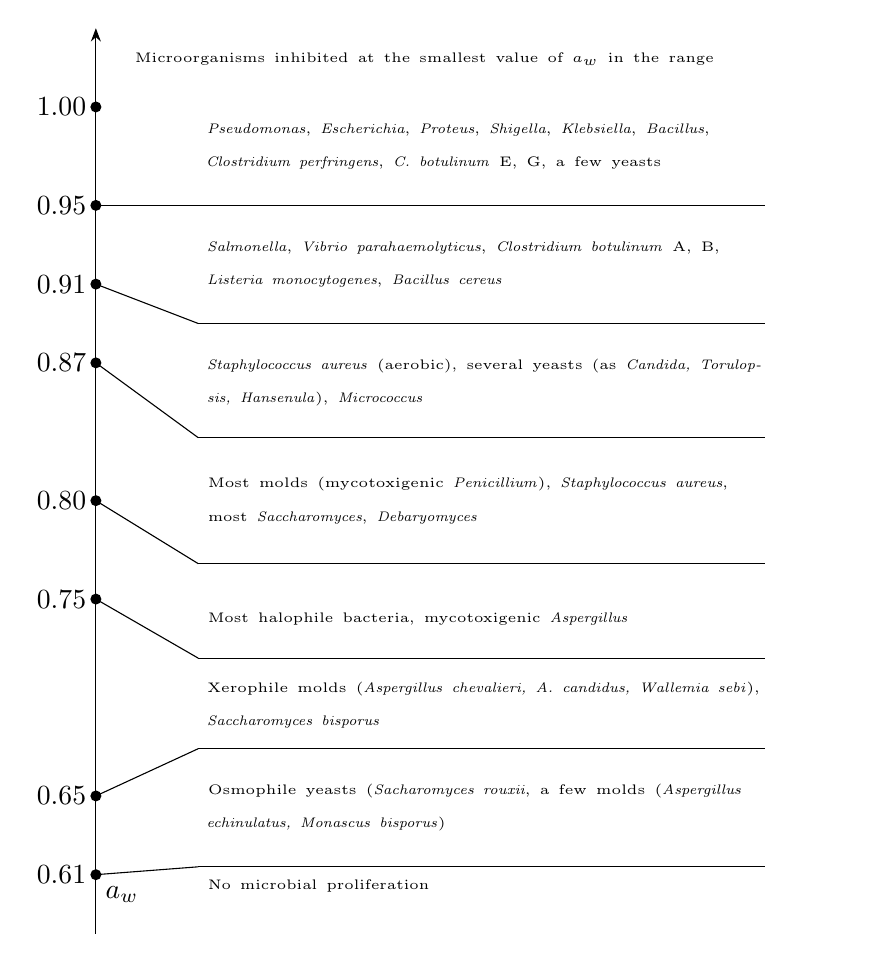
\begin{tikzpicture}[>=Stealth]
		\draw[->] (5,-0.5) -- (5,11);
		\draw (5,0.0) node[anchor=west] {$a_w$};
		\draw (5,8.75) -- (6.3,8.75);
		\draw (6.3,8.75) -- (13.5,8.75);
		\draw (5,7.75) -- (6.3,7.25);
		\draw (6.3,7.25) -- (13.5,7.25);
		\draw (5,6.75) -- (6.3,5.8);
		\draw (6.3,5.8) -- (13.5,5.8);
		\draw (5,5) -- (6.3,4.2);
		\draw (6.3,4.2) -- (13.5,4.2);
		\draw (5,3.75) -- (6.3,3);
		\draw (6.3,3) -- (13.5,3);
		\draw (5,1.25) -- (6.3,1.85);
		\draw (6.3,1.85) -- (13.5,1.85);
		\draw (5,0.25) -- (6.3,0.35);
		\draw (6.3,0.35) -- (13.5,0.35);
		\fill[black] (5,0.25) circle (0.07);
		\fill[black] (5,1.25) circle (0.07);
		\fill[black] (5,3.75) circle (0.07);
		\fill[black] (5,5) circle (0.07);
		\fill[black] (5,6.75) circle (0.07);
		\fill[black] (5,7.75) circle (0.07);
		\fill[black] (5,8.75) circle (0.07);
		\fill[black] (5,10) circle (0.07);
		\draw (10,10.4) node[anchor=south, text width=9cm]
		{\tiny{Microorganisms inhibited at the smallest value of
		$a_w$ in the range}};
		\draw (6.3,9.5) node[anchor=west, text width=7cm]
		{\tiny{\textit{Pseudomonas}, \textit{Escherichia},
		\textit{Proteus}, \textit{Shigella}, \textit{Klebsiella},
		\textit{Bacillus}, \textit{Clostridium perfringens},
		\textit{C. botulinum} E, G, a few yeasts}};
		\draw (6.3,8) node[anchor=west, text width=7cm]
		{\tiny{\textit{Salmonella}, \textit{Vibrio parahaemolyticus},
		\textit{Clostridium botulinum} A, B, \textit{Listeria
		monocytogenes}, \textit{Bacillus cereus}}};
		\draw (6.3,6.5) node[anchor=west, text width=7cm]
		{\tiny{\textit{Staphylococcus aureus} (aerobic), several
		yeasts (as \textit{Candida, Torulopsis, Hansenula}),
		\textit{Micrococcus}}};
		\draw (6.3,5) node[anchor=west, text width=7cm]
		{\tiny{Most molds (mycotoxigenic \textit{Penicillium}),
		\textit{Staphylococcus aureus},
		most \textit{Saccharomyces}, \textit{Debaryomyces}}};
		\draw (6.3,3.5) node[anchor=west, text width=7cm]
		{\tiny{Most halophile bacteria,
		mycotoxigenic \textit{Aspergillus}}};
		\draw (6.3,2.4) node[anchor=west, text width=7cm]
		{\tiny{Xerophile molds (\textit{Aspergillus chevalieri, A.
		candidus, Wallemia sebi}), \textit{Saccharomyces bisporus}}};
		\draw (6.3,1.1) node[anchor=west, text width=7cm]
		{\tiny{Osmophile yeasts (\textit{Sacharomyces rouxii},
		a few molds (\textit{Aspergillus echinulatus, Monascus
		bisporus})}};
		\draw (6.3,0.1) node[anchor=west, text width=7cm]
		{\tiny{No microbial proliferation}};
		\draw (5,0.25) node[anchor=east] {0.61};
		\draw (5,1.25) node[anchor=east] {0.65};
		\draw (5,3.75) node[anchor=east] {0.75};
		\draw (5,5) node[anchor=east] {0.80};
		\draw (5,6.75) node[anchor=east] {0.87};
		\draw (5,7.75) node[anchor=east] {0.91};
		\draw (5,8.75) node[anchor=east] {0.95};
		\draw (5,10) node[anchor=east] {1.00};
	\end{tikzpicture}
	\caption{$a_w$ values for microbial growth}
	\label{fig:germ}
\end{figure}

In the conditions usually found in the food industry, is reasonable to assume
that the gas phase of the system behaves as an ideal gas\cite{canovas2007},
in most situations. Furthermore, the reference condition is taken as pure and liquid
water at the same pressure and temperature as the system. Therefore, one can obtain:

\begin{equation}
	\label{eq:def_atv}
	a_w \equiv \left(\cfrac{f_w}{f^\text{ref}_w}\right)_T%
		\approx \left(\cfrac{p^\text{vap}_w}{p^\text{vap,ref}_w}\right)_T
\end{equation}

For ideal solutions, the evaluation of water activity is straightforward: for all
component $u$ in a mixture, its activity $a_i$ is simply its molar fraction $x_i$;
hence, $a_w = x_w$. However, not all systems are ideal, and therefore one needs to
adopt another property, the activity coefficient of the water, $\gamma_w$:

\begin{equation}
	a_w = \gamma_wx_w \implies \gamma_w = \cfrac{a_w}{x_w}
\end{equation}

Yet, even if one now has an indicator of the deviation of a solution from
ideality , another problem arises: the activity coefficient is not a good
parameter to evaluate the deviations when applied to very diluted solutions;
after all, $a_w=a_w(x_w)$ is a continuous function, and as the solution is diluted,
$a_w$ must go to 1 (because the limit $x_w=1$ is the reference solution), and
therefore one will observe that:

\begin{equation}
	\lim_{x_w \to 1}\gamma_w = 1
\end{equation}

And for many solutions of interest, one can observe not only high deviations from
ideal behavior, but also extremely diluted solutions. Thus, one adopts another
property, the osmotic coefficient $\phi$, defined as:

\begin{equation}
	\phi = \cfrac{\ln(a_w)}{\ln(x_w)}
\end{equation}

One can compare these two properties and visualize a possible behavior of
the water activity as the composition of a mixture changes by observing
the data plotted in the figure \ref{fig_atv_gamma_gluc} \cite{ebrahimi2016}.

\begin{figure}[h]
	\centering
	\begin{tikzpicture}
		\newsavebox{\minigrafglic}
		\savebox{\minigrafglic}{%
		\scalebox{0.5}{%
		\begin{tikzpicture}
			\begin{axis}[
			xmin=0.97,xmax=1.0,
			ymin=0.97,ymax=1.0,
			x dir=reverse,
			width=7cm,
			height=7cm,
			xlabel = {$x_w$},
			ylabel = {$a_w$},
			]
			\addplot+[
				color=pverydarkred,
				mark=o,
				only marks,
			]
			table[x={xw},y={aw}]{glucose_a_w_and_phi.dat};
			\addlegendentry{$a_w$ (experimental)};
			\addplot+[
				color=black,
				no marks,
				domain=0.96:1.0,
				samples=5,
			]{x};
			\addlegendentry{$a_w=x_w$};
		\end{axis}
	\end{tikzpicture}
	}}
	\begin{axis}[
			xmin = 0.97, xmax = 1.0, xlabel = {$x_w$},
			ymin = 0.96, ymax = 1.05, ylabel = {$\phi$},
			x tick label style={
				/pgf/number format/.cd,
				fixed,
				fixed zerofill,
				precision=3,
				/tikz/.cd
			},
			y tick label style={
				/pgf/number format/.cd,
				fixed,
				fixed zerofill,
				precision=3,
				/tikz/.cd
			},
			legend pos = south west,
			axis y line=left,
			x axis line style={-},
			xlabel near ticks,
			ylabel near ticks,
			x dir=reverse,
			ytick={0.97,0.985,1.00,1.015,1.03,1.045},
		]
		\addplot+[
			color=pdarkblue,
			mark=square,
			very thick,
			only marks,
		]
		table[x={xw},y={phi}]{glucose_a_w_and_phi.dat};
		\addlegendentry{$\phi$};
		\draw (axis cs: 0.981,0.99)node{\usebox{\minigrafglic}};
		\end{axis}
		\begin{axis}[
			xmin = 0.97, xmax = 1.0, xlabel = {$x_w$},
			ymin = 0.9977, ymax = 1.0001, ylabel = {$\gamma_w$},
			y tick label style={
				/pgf/number format/.cd,
				fixed,
				fixed zerofill,
				precision=4,
				/tikz/.cd
			},
			axis y line=right,
			axis x line=none,
			legend pos = south east,
			x dir=reverse,
		]
		\addplot+[
			color=pverybrightred,
			mark=o,
			very thick,
			only marks,
		]
		table[x={xw},y={gammaw}]{glucose_a_w_and_phi.dat};
		\addlegendentry{$\gamma_w$};
		\end{axis}
	\end{tikzpicture}
	\caption{Activity ($a_w$), Activity coefficient ($\gamma_w$) and%
	osmotic coefficient ($\phi$) of water in D-glucose solutions. %
	One should observe the difference in the $\gamma_w$ and $\phi$ axis scales.}
	\label{fig_atv_gamma_gluc}
\end{figure}

In addition, one must remember that water activity measurements are sometimes
obtained indirectly; instead of measurements of vapor pressure in the system
and comparison with the same property in the reference system (as shown in the
equation \ref{eq:def_atv}), one can measure properties as freezing point
depression, boiling point elevation, or the composition of another solution
in osmotic equilibrium with the system under analysis.

For instance, a few data sets obtained for $n$-ary solutions of carbohydrates
\cite{abderafi1994} are, in fact, boiling point elevation data. Hence, the
experimental measurements must first be converted to osmotic coefficient data,
through the equations \ref{eq:eleb_to_osco} \cite{ge2009,ge2009err}, which are
plotted in the figure \ref{fig_ge_and_wang}.

\begin{equation}
	\label{eq:eleb_to_osco}
	\begin{cases}
		\ln(a_w) = -\cfrac{\Delta H^\text{vap}_{0,T_B}\left(\cfrac{1}{T_B}%
			-\cfrac{1}{T_B+\Delta T_B}\right)-%
			\Delta C_p^\text{vap}\Bigg[\ln\left(\cfrac{T_B+%
			\Delta T_B}{T_B}\right) - \cfrac{\Delta T_B}{T_B+%
			\Delta T_B}\Bigg]}{R}\\
		\ln(a_w) = \cfrac{\Delta H^\text{fus}_{0,T_F}\left(\cfrac{1}{T_F}-%
		\cfrac{1}{T_F-\Delta T_F}\right)+\Delta C_p^\text{fus}%
		\Bigg[\ln\left(\cfrac{T_F-\Delta T_F}{T_F}\right) -%
		\cfrac{\Delta T_F}{T_F-\Delta T_F}\Bigg]}{R}
	\end{cases}
\end{equation}

\begin{figure}[h]
	\centering
	\begin{subfigure}{0.5\textwidth}
		\begin{tikzpicture}[scale=0.75]
			\begin{axis}[
				ylabel={$a_w$},
				xlabel={$T_B$[\textcelsius]},
				ymax=1, xmax=115, xmin=100,
			]
				\addplot [
					color=pred,
					no marks,
					very thick,
				]
					table [x={BPE},y={aw},col sep=comma]
						{ge_and_wang_bpe.csv};
			\end{axis}
		\end{tikzpicture}
		\caption{Boiling Point}
	\end{subfigure}%
	\hfill%
	\begin{subfigure}{0.5\textwidth}
		\begin{tikzpicture}[scale=0.75]
			\begin{axis}[
				ylabel={$a_w$},
				xlabel={$T_F$[\textcelsius]},
				ymax=1, xmin=-15, xmax=0,
			]
				\addplot [
					color=pblue,
					no marks,
					very thick,
				]
					table [x={FPD},y={aw},col sep=comma]
						{ge_and_wang_fpd.csv};
			\end{axis}
		\end{tikzpicture}
		\caption{Freezing Point}
	\end{subfigure}
	\caption{Relation between $T_B$/$T_F$ (in \textcelsius) and $a_w$, %
		$P=P_\text{atm}$}
	\label{fig_ge_and_wang}
\end{figure}


With $\Delta C_p$ defined as the difference in specific heat between the
phases: $\Delta C_p^\text{vap} = C_p^\text{vapor} -%
C_p^\text{liquid}$ and $\Delta C_p^\text{fus} = C_p^\text{liquid} -%
C_p^\text{solid}$, $\Delta T_F$ defined as the freezing point depression,
$\Delta T_B$ the boiling point elevation and $\Delta H_{0,T_B}^\text{vap}$ and
$\Delta H_{0,T_F}^\text{fus}$ representing the enthalpies of vaporization and fusion
of the solvent at $T_B$/$T_F$.



\part{Bibliographic Revision}

\chapter{Water activity modelling}

\section{Analysed models}

Several models were analysed, ranging in complexity from simple as Raoult's Law
or Caurie's equation to complex as the iterative procedure derived from the
Zdanovskii's relation or the UNIQUAC model, for subsequent comparison with a
virial equation (as in \ref{eq:ad_pessoa}, adapted from \cite{pessoa2008}, in
which $b_i$ and $c_{ij}$ are adjustable parameters and $\theta$ is a measure
of concentration).

\begin{equation}
	\label{eq:ad_pessoa}
	\ln(a_w) = \sum_{i \neq w}\theta_i\Bigg(1 +%
	2b_i+3\sum_{j \neq w}c_{ij}\theta_j\Bigg)
\end{equation}

For obtaining $a_w$ values in binary solutions, one has several distinct models
to choose from. From those models, the following shall be analysed and compared:

\begin{itemize}
	\item Raoult's Law: Simplest model, for ideal solutions. Assumes
		water activity $a_w = x_w$, its molar fraction;
	\item Norrish's Equation \cite{norrish1966}: Raoult's Law, corrected.
		One can, with the molar fraction of water, $x_w$, molar
		fraction of the other substance, $x_s$, and one adjustable
		parameter ($K$), utilize the equation \ref{eq_norrish} to
		obtain the water activity of a solution.
		\ref{eq_norrish}:
		\begin{equation}
			\label{eq_norrish}
			a_w = x_w\exp\Big[\Big(\sqrt{K}x_s\Big)^2\Big]
		\end{equation}
	\item UNIQUAC (\textit{universal quasi-chemical}) Model
		\cite{abrams1975}: Possibly the most complex model among the
		chosen ones; requiring two adjustable parameters for each pair
		of substances present in the mixture (between solvents and
		solutes), can be used for binary or $n$-ary systems. Even though
		the nonlinear fitting for the model presents a high computational
		cost, as we are dealing with simple mixtures (with a maximum of
		four components), the complexity of the model is not a problem.
\end{itemize}

For $n$-ary solutions, a few other models were chosen for analysis and
comparisons:

\begin{itemize}
	\item Raoult's Law: water activity $a_w$ equals $x_w$,
		its molar fraction;
	\item Norrish's Equation: adopted with a small modification to the equation
		\ref{eq_norrish}, as shown in the equation \ref{eq_norrish_multi};
		\begin{equation}
			\label{eq_norrish_multi}
			a_w = x_w\exp\Big[\Big(\sum_{i \neq w}%
			\sqrt{K_i}x_i\Big)^2\Big]
		\end{equation}
	\item Caurie's Model \cite{caurie1986}: water activity as a correction
		of the product of the water activities of binary solutions
		in which each component's molalities are either zero or equal
		to its molality in the solution of interest, as presented
		in the equation \ref{eq_caurie}, in which $a_{wi}$ is the
		water activity in a binary solution in which the molality $m_i$
		of the substance $i$ remains the same and $n$ is the total number
		of solutes in the mixture.
		\begin{equation}
			\label{eq_caurie}
			a_w = \prod_{i \neq w}a_{wi}-\left[\cfrac{n}%
			{55.5^2}\sum_{\substack{i \neq j \\ i,j \neq w}}%
			m_im_j + \cfrac{(n+1)}{55.5^3}\sum_{%
			\substack{i\neq j,k \\ j \neq k \\  i,j,k \neq w}}%
			m_im_jm_k\right]
		\end{equation}
		To obtain the water activities of the binary solutions,
		we assumed ideal solution (Raoult's Law).
	\item Zdanovskii's Relation \cite{chen1973,sangster1973}:
		applied for ternary mixtures only, it's an iterative process
		based in the Zdanovskii relation; for a ternary mixture with
		two generic solutes 1 and 2, we adopt two binary solutions, one
		with 1 as its only solute, the other with 2, in osmotic equilibrium
		with the solution of interest. With $m_{01}$ and $m_{02}$ as the
		molalities of each solute in each the binary solution, and
		$m_1$ and $m_2$ as the molalities of each solute in the solution
		of interest, the Zdanovskii's relation ($m_1m_{01}^{-1} +
		m_2m_{02}^{-1} = 1$) generates an iterative procedure that
		returns the water activity of a ternary mixture from the
		curves $a_w=a_w(x_w)$ of binary mixtures of each solute.
	\item UNIQUAC (\textit{universal quasi-chemical}) Model, previously
		cited.
\end{itemize}

\section{Applicability of the models to the samples}

Since one is not only interested in fitting curves to data sets, but also in
assessing the possibility of predicting water activities for $n$-ary systems
based on data from binary systems, one can split the available models in two
great groups. For a thermodynamical model (as shown in equation
\ref{eq:geral_bigphi}) with $N$ parameters $(A_j)_{j \in \{1, 2, \ldots N\}}$
for the osmotic coefficient in a system of composition given by the molar
fractions of each component $(x_i)_\text{$i$ component}$, at temperature $T$
and pressure $P$, one can obtain estimates $(A^*_j)_{j \in \{1, 2, \ldots N\}}$
for the parameters through the use of nonlinear least-squares fitting,
as shown in equation \ref{eq:min_quad}, for a set of $K > N$ experimental data
points
$\{(\phi^k, T^k, P^k, (x_i)^k_\text{$i$ component}), k \in \{1,2,\ldots,K\}\}$.

\begin{equation}
	\label{eq:geral_bigphi}
	\phi = \Phi((A_j)_{j \in \{1, 2, \ldots, N\}}, (x_i)_\text{$i$ %
		component of the mixture}, T, P)
\end{equation}

\begin{equation}
	\label{eq:min_quad}
	\minimize_{(A_j^*)_{j \in \{1,2,\ldots,N\}} \in \mathbb{R}^N}%
	\left(\sum_{k \in \{1,2,\ldots,K\}}\left[\phi^k - \Phi((A^*_j)_{j%
	\in \{1, 2, \ldots, N\}}, (x^k_i)_\text{$i$ component},%
	T^k, P^k)\right]^2\right)
\end{equation}

For data obtained exclusively from binary systems, one may write:

\begin{equation}
	\forall k \in \{1,2,\ldots,K\} \;\; \exists i \neq w%
	\text{ component } : \forall \;\; i' \neq i, i' \neq w\;\; x^k_{i'} = 0
\end{equation}

When for all sets of data obtained exclusively from binary systems the equation
\ref{eq:no_bin_fit} is valid, one can say that the model presents an adjustable
parameter of component-component interaction. Otherwise, one can say that the model
has no parameters accounting for the interaction between two components.

\begin{equation}
	\label{eq:no_bin_fit}
	\exists j' \in \{1,2,\ldots,N\} : \forall \alpha \in \mathbb{R}\;\;%
	(A_j^*)_{j \in \{1,2,\ldots,N\}, A_{j'}^* = \alpha}%
	\text{ is a solution of \ref{eq:min_quad}}
\end{equation}

One must differentiate these two groups, for one of the aims of the project
is the assessment of the applicability of parameter estimates, obtained through
fitting curves through binary data, to $n$-ary data; this is important, primarily
because experimental data for binary systems are more abundant and easier to
obtain, but also due to the high computational cost in multivariate nonlinear
fitting.

An example of a model in the second category is the one proposed by Norrish; also,
one could trivially place models such as Zdanovskii's procedure and Caurie's
relation in the category. For the first one, more complex, the virial model defined
in the equation \ref{eq:ad_pessoa} or the UNIQUAC model can be considered as
examples.

\section{Limitations of the models and problems found}

One of the main problems found is the simple non-applicability of some models
to a few sets of data; as an example, one may check the intrinsical limitations
of the Norrish's model.

Norrish's model, as seen in the equations \ref{eq_norrish} and
\ref{eq_norrish_multi}, can be algebraically manipulated to yield equation
\ref{eq_phi_norrish} for the calculation of the osmotic coefficient $\phi$.

\begin{equation}
	\label{eq_phi_norrish}
	\phi = \cfrac{\ln(a_w)}{\ln(x_w)} = \cfrac{\ln(x_w) + \left(\sum_{ i\neq w}
	\sqrt{K_i}x_1\right)^2}{\ln(x_w)}
\end{equation}

As $x_w \le 1 \implies \ln(x_w) \le 0$, one can observe that the model can't
predict a value for $\phi$ greater than 1; however, this is not verified
in all real solutions, that can show several behaviors, ranging from
monotonically decreasing functions (as the model requires,\footnote{%
	Since $\lim_{x_w \to 1}\phi_\text{Norrish} = 1$.
} to monotonically increasing functions, the opposite of the desired
behavior, which can be seen in figure \ref{fig_atv_gamma_gluc}
and, more clearly, in figure \ref{fig_manose_phi}.

Another example is Caurie's equation; since $\lim_{x_w \to 0}m_i = +\infty$,
one can observe the existence of crtical dilutions, beyond which the
model simply fails to return a physically meaningful result, because
$a_w \in [0,1]$ and, as shown in the equations \ref{eq_caurie_fail},
there are values for the molar fractions of each component in the mixture
that, according to the model, must force the system to exhibit negative
values of $a_{w,\text{Caurie}}$. Besides, as the molar fraction of water
in a mixture decreases, $\phi$ must, in the limit, be as close as
desired to 0.

\begin{equation}
	\label{eq_caurie_fail}
	\begin{split}
		a_{w,\text{Caurie}} = \prod_{i \neq w}a_{w,i} - \left[\cfrac{n}%
			{55.5^2}\sum_{\substack{i \neq j \\ i,j \neq w}}%
			m_im_j + \cfrac{(n+1)}{55.5^3}\sum_{%
			\substack{i\neq j,k \\ j \neq k \\  i,j,k \neq w}}
			m_im_jm_k\right] <\\
		1 - \cfrac{n}{55.5^3}\left[55.5 \times%
			\sum_{\substack{i \neq j \\ i,j \neq w}}%
			m_im_j + \cfrac{n+1}{n}\sum_{%
			\substack{i\neq j,k \\ j \neq k \\  i,j,k \neq w}}
			m_im_jm_k\right]\implies\\
		\lim_{\substack{m_k \to +\infty \\%
				\forall n \neq k, \text{ $m_n$ constant}}}%
			a_{w,\text{Caurie}} = -\infty \implies%
		\lim_{x_w \to 0} a_{w,\text{Caurie}} = -\infty
	\end{split}
\end{equation}

This diversity of behaviors can be useful. For instance, for the virial model,
the measure chosen for the concentration was molar concentration, since one can
show that the data rarely follow the curves to which they are restricted when
one utilizes instead the molar fraction, as one would naïvely do. This can be
seen in the equations \ref{eq_phi_virial_mono_frac}
\footnote{%
	This can be affirmed since, $\forall w > 0$:
	\begin{equation*}
		\begin{split}
			e^w = 1 + w + \cfrac{w^2}{2!} + \ldots \ge w +1
			\stackrel{(z = w+1)}{\implies} e^z \ge ze \implies
				z \ge \ln(z) + 1
			\stackrel{\left(y=\cfrac{1}{z}\right)}{\implies}
				\cfrac{1}{y} \ge
				\ln\left(\cfrac{1}{y}\right) + 1 \implies\\
			1-y \ge y\ln\left(\cfrac{1}{y}\right)
			\stackrel{(x=1-y)}{\implies} x >
				(1-x)\ln\left(\cfrac{1}{1-x}\right)\implies
			\cfrac{x}{1-x} + \ln(1-x) > 0 \implies\\
				\cfrac{d}{dx}\left(\cfrac{x}{\ln(1-x)}\right) > 0
		\end{split}
	\end{equation*}
}
for binary systems, with $x$ as the molar fraction of the solute: the model
(with $\theta_i = x_i$) is obligatorily a monotonic function.

\begin{equation}
	\label{eq_phi_virial_mono_frac}
	\begin{split}
		\ln(a_w) = -x + 2bx \implies \phi =
			\cfrac{-x + 2bx}{\ln(1-x)}\implies\\
		\phi = (2b-1)\cfrac{x}{\ln(1-x)} \implies
			\forall (x_1,x_2) \in (0,1)\times(0,1)\;\;
			\cfrac{d\phi}{dx}\Big|_{x_1} \times
			\cfrac{d\phi}{dx}\Big|_{x_2} \ge 0
	\end{split}
\end{equation}

Another challenge (not intrinsical to the models, but specific to the data)
is the distribution of the data in small sets, compared to the amount of
data points required to fit a large model (as the complete UNIQUAC model,
for instance). Indeed, for a mixture of $n$ components, the model requires
$2n+n^2 \in \mathcal{O}(n^2)$ parameters (accounting for the interaction
energies $U_{ij}$ and the parameters $r_i$ and $q_i$. To solve this problem,
a few simplifications, from the literature, were adopted, as exhibited in
the equations \ref{eq_uniquac_simpl}.

\begin{equation}
	\label{eq_uniquac_simpl}
	\begin{cases}
		u_{ij} = \sqrt{u_{ii}u_{jj}}\\
		r_i = q_i
	\end{cases}\forall\ i, j\text{ component}
\end{equation}

Additionally, one must consider that a non-negligible amount of the datasets
exhibits colinearity-related problems, which, even if not a problem for correlation,
makes the values of the parameters adjusted to the data set less reliable. Finally,
for very diluted solutions, one can observe that the osmotic coefficient values
have big uncertainties, due to the relatively high uncertainties in the measures
of the logarithm of numbers close to 1.

\begin{figure}[h]
	\centering
	\begin{tikzpicture}
		\newsavebox{\minigrafmann}
		\savebox{\minigrafmann}{%
		\scalebox{0.5}{%
		\begin{tikzpicture}
			\begin{axis}[
			xmin=0.0,xmax=0.07,
			ymin=0.93,ymax=1.0,
			width=7cm,
			height=7cm,
			xlabel = {$x$},
			ylabel = {$a_w$},
			xlabel near ticks,
			ylabel near ticks,
			xticklabel style={
				/pgf/number format/fixed,
				/pgf/number format/precision=3,
				/pgf/number format/fixed zerofill
			},
			scaled x ticks=false,
			]
			\addplot+[
				color=pbrightred,
				mark=o,
				only marks,
				thick,
			]
			table[x={mannose},y={aw_exp},col sep=comma]
				{ebrahimi_mannose_norrish.csv};
			\addplot+[
				color=pverybrightblue,
				no marks,
				thick,
			]
			table[x={mannose},y={aw_calc},col sep=comma]
				{ebrahimi_mannose_norrish.csv};
			\addplot+[
				color=pblue,
				no marks,
				thick,
			]
			table[x={mannose},y={aw_calc},col sep=comma]
				{ebrahimi_mannose_virial.csv};
			\addplot+[
				color=pverydarkblue,
				no marks,
				thick,
			]
			table[x={mannose},y={aw_calc},col sep=comma]
				{ebrahimi_mannose_uniquac.csv};
		\end{axis}
	\end{tikzpicture}
	}}
	\begin{axis}[
			xmin = 0.0, xmax = 0.072, xlabel = {$x_\text{mannose}$},
			ymin = 0.975, ymax = 1.029, ylabel = {$\phi$},
			legend pos = south east,
			xlabel near ticks,
			ylabel near ticks,
			xticklabel style={
				/pgf/number format/fixed,
				/pgf/number format/precision=3,
				/pgf/number format/fixed zerofill
			},
			scaled x ticks=false,
			xtick = {0.015,0.030,0.045,0.060},
		]
		\addplot+[
			smooth,
			color=pverybrightblue,
			no marks,
			thick,
		]
		table[x={mannose},y={phi_calc},col sep=comma]
			{ebrahimi_mannose_norrish.csv};
		\addlegendentry{Norrish};
		\addplot+[
			smooth,
			color=pblue,
			no marks,
			thick,
		]
		table[x={mannose},y={phi_calc},col sep=comma]
			{ebrahimi_mannose_virial.csv};
		\addlegendentry{virial};
		\addplot+[
			smooth,
			color=pverydarkblue,
			no marks,
			thick,
		]
		table[x={mannose},y={phi_calc},col sep=comma]
			{ebrahimi_mannose_uniquac.csv};
		\addlegendentry{UNIQUAC};
		\addplot+[
			color=pbrightred,
			mark=o,
			very thick,
			only marks,
		]
		table[x={mannose},y={phi_exp},col sep=comma]
			{ebrahimi_mannose_uniquac.csv};
		\addlegendentry{experimental};
		\draw (axis cs:0.018,1.015) node{\usebox{\minigrafmann}};
		\end{axis}
	\end{tikzpicture}
	\caption{Osmotic coefficient $\phi$ e adjusted models for a mannose solution}
	\label{fig_manose_phi}
\end{figure}


\chapter{Experimental data sets analysed}

\label{sec_selec_data}

Due to external circunstances, laboratorial experiments are neither safe nor
practical; fortunately, they are also not needed: the previous research on the
area is rich enough to supply a good selection of experimental data for binary
and/or multicomponent systems. The data used in the project and its sources are
listed below.

\begin{itemize}
	\item For binary systems:
		\begin{itemize}
			\item Abderafi \& Bounahmidi (1994) \cite{abderafi1994};
			\item Bhandari \& Bareyre (2003) \cite{bhandari2003},
				direct measurements of $a_w$ for solutions of water
				and glucose at 25\textcelsius, with values between
				$x_w = 0.808$ and $x_w = 0.917$;
			\item Bonner (1982) \cite{bonner1982}, osmotic coefficient
				and activity measurements for lisine
				and arginine at a temperature of 298.15K.
			\item Chen (1987) \cite{chen1987}, water activity
				measurements of a few solutions of carbohydrates
				obtained through equilibrium relative humidity, at
				freezing temperatures.
			\item Cooke, Jónsdóttir \& Westh (2002) \cite{cooke2002a},
				vapor pressure measurements at temperatures of
				24.91\textcelsius\ and 44.84\textcelsius, for
				sucrose and other carbohydrates, with molar fractions
				between 0 and 0.24.
%			\item Dunning, Evans \& Taylor (1951) \cite{dunning1951},
%				medidas de pressão de vapor da água para soluções de
%				sacarose com temperaturas entre 60 e
%				95\textcelsius\ e frações molares $x_w$ entre 0.79
%				e 0.96.\footnote{%
%					Não puderam ser utilizados, tendo em vista
%					que foram, todos, obtidos a temperaturas
%					distintas, \textit{i.e.} não é coerente
%					ajustar esse conjunto de dados com uma
%					isoterma.
%				}
			\item Ebrahimi \& Sadeghi (2016) \cite{ebrahimi2016},
				osmotic coefficient data for several carbohydrates,
				including monosaccharides, dissacharides,
				trissacharides and polyols, at 308.15K.
			\item Ellerton, Reinfelds, Mulcahy \& Dunlop (1964)
				\cite{ellerton1964} osmotic pressure measurements
				obtained through the isopiestic method for five
				aminoacids at the temperature of 25\textcelsius.
			\item Himanshu, Priyanka \& Anakshi (2005)
				\cite{himanshu2005}, freezing point depression
				measurements were converted to osmotic coefficient
				data for diluted binary solutions of nine aminoacids
				(glycine, L-serine, L-proline, DL-valine,
				DL-alanine, L-threonine, hidroxy-L-proline,
				L-isoleucine and DL-methionine).
			\item Kiyosawa (1992) \cite{kiyosawa1992}, freezing
				point depression measurements of binary polyol
				solutions
			\item Kuramochi, Noritomi, Hoshino \& Nagahama (1997)
				\cite{kuramochi1997}, activity coefficient
				measurements for four aminoacids (glycine,
				L-alanine, L-serine and L-valine), at 298.15K
			\item Maximo, Meirelles \& Batista (2010) \cite{maximo2010},
				activity coefficient measurements obtained through
				boiling point elevation for sucrose, fructose and
				glucose at different pressures.
			\item Ninni \& Meirelles (2001) \cite{ninni2001}, direct
				measurements of water activity for binary solutions
				of four aminoacids (glycine, DL-alanine, L-proline
				and L-arginine), at 25\textcelsius.
			\item Pinho (2008) \cite{pinho2008}, direct water activity
				measurements for solutions of three aminoacids
				(glycine, DL-alanine and L-serine) at
				25\textcelsius\ and $x_w$ values close to 1.
			\item Romero \& González (2006) \cite{romero2006}, osmotic
				coefficient measurements obtained through the
				isopiestic method, for glycine, DL-$\alpha$-alanine
				and DL-$\alpha$-aminobutyric acid, at temperatures
				ranging from 288.15K and 303.15K.
			\item Tsurko, Neueder \& Kunz (2007) \cite{tsurko2007},
				osmotic coefficient data for three aminoacid
				solutions (glycine, glutamic acid and histidine),
				obtained through vapor-liquid equilibria, at
				temperatures of 298.15K and 310.15K.
			\item Velezmoro, Oliveira, Cabral \& Meirelles (2000)
				\cite{velezmoro2000}.
		\end{itemize}
	\item For $n$-ary systems:
		\begin{itemize}
			\item Abderafi \& Bounahmidi (1994) \cite{abderafi1994},
				boiling point elevation data for binary, ternary
				and quaternary solutions of sucrose, glucose and
				fructose, at low dilutions and atmospheric pressure.
			\item Norrish (1966) \cite{norrish1966}, equilibrium
				relative humidity measurements for ternary solutions
				of water, sucrose and sorbitol, glycerol or dextrose,
				at 25\textcelsius.
			\item Robinson \& Stokes (1961) \cite{stokes1961},
				osmotic equilibria data for ternary solutions
				of sucrose and mannitol at 25\textcelsius.
			\item Stokes \& Robinson (1966) \cite{stokes1966},
				osmotic equilibria data of ternary solutions with
				sucrose as a solute.
			\item Velezmoro, Oliveira, Cabral \& Meirelles (2000)
				\cite{velezmoro2000}, direct $a_w$ measurements
				at temperaturas of 25, 30 and 35\textcelsius\ for
				glucose, fructose, sucrose and maltose binary and
				quaternary solutions at high dilutions.
		\end{itemize}
\end{itemize}

\begin{tabularx}{\textwidth}{ X  c  X }
	\caption{Data points distribution by source (binary systems)}
	\label{tab_dados_pontos}\\
	\toprule
	Reference & \textnumero\ of points & Method utilized\\
	\midrule
	\endfirsthead
	\toprule
	Reference & \textnumero\ of points & Method utilized\\\hline
	\midrule
	\endhead
	\midrule
	\multicolumn{3}{r}{\footnotesize(Continue in the following page)}
	\endfoot
	\endlastfoot
	Abderafi \& Bounahmidi (1994) & 36 & Vapor-liquid equilibria\\
	Bhandari \& Bareyre (2003) & 10 & Direct $a_w$ measurements\\
	Bonner (1982) & 34 & Isopiestic method\\
	Chen (1987) & 14 & Vapor pressure measurements\\
	Cooke, Jónsdóttir \& Westh (2002) & 40 & Vapor pressure measurements\\
%	Dunning, Evans \& Taylor (1951) & 102 & Medições de pressão de vapor\\
	Ellerton, Reinfelds, Mulcahy \& Dunlop (1964) & 91 & Isopiestic method\\
	Ebrahimi \& Sadeghi (2016) & 246 & Vapor pressure osmometry\\
	Himanshu, Priyanka \& Anakshi (2005) & 45 &
		Freezing point depression\\
	Kiyosawa (1992) & 49 & Freezing point depression\\
	Kuramochi, Noritomi, Hoshino \& Nagahama (1997) & 44 &
		Vapor pressure measurements\\
	Maximo, Meirelles \& Batista (2010) & 168 & Boiling point elevation\\
	Ninni \& Meirelles (2001) & 31 & Vapor pressure measurements\\
	Pinho (2008) & 75 & Direct $a_w$ measurements\\
	Romero \& González & 144 & Isopiestic method\\
	Robinson \& Stokes (1961) & 43 & Isopiestic method\\
	Tsurko, Neueder \& Kunz (2007) & 57 & Vapor pressure measurements\\
	Velezmoro, Oliveira, Cabral \& Meirelles (2000) &
		145 & Vapor pressure measurements\\\hline
	Total & \multicolumn{2}{c}{1251}\\\hline
\end{tabularx}

\begin{tabularx}{\textwidth}{ X  c  X }
	\caption{Data points distribution by source ($n$-ary systems)}
	\label{tab_dados_multi_pontos}\\
	\toprule
	Reference & \textnumero\ of points & Method utilized\\
	\midrule
	\endfirsthead
	\toprule
	Reference & \textnumero\ of points & Method utilized\\\hline
	\midrule
	\endhead
	\midrule
	\multicolumn{3}{r}{\footnotesize(Continue in the following page)}
	\endfoot
	\endlastfoot
	Abderafi \& Bounahmidi (1994) & 174 & Boiling point elevation\\
	Norrish (1966) & 26 & Vapor pressure measurements\\
	Robinson \& Stokes (1961) & 74 & Isopiestic method\\
	Stokes \& Robinson (1966) & 24 & Isopiestic method\\
	Velezmoro, Oliveira, Cabral \& Meirelles (2000) & 135 &
		Vapor pressure measurements\\\hline
	Total & \multicolumn{2}{c}{358}\\\hline
\end{tabularx}



\part{Computational tools}

\chapter{Choice of computational tools}

The least-squares method was utilized for the nonlinear fitting of the models
to the experimental data sets. This was achieved with a program in the \texttt{C}
programming language, utilizing the functions and routines of the GNU Scientific
Library (GSL), a library for numerical computations under the GNU General Public
License \cite{galassi_book}. The choice of this library for nonlinear optimizations
was due to the ease of access of the intermediate steps in the iterative calculations
of the desired parameters.

\chapter{Property conversion}

Unfortunately, not all data sets utilized were available as series of $a_w$ values
as a function of composition; as seen in the tables \ref{tab_dados_pontos} and
\ref{tab_dados_multi_pontos}, one must, initially, convert all data to the same
basis, before supplying the data to the program responsible for fitting. The basis
of choice was simply water activity as a function of molar fraction, with all
conversion of the activity data to osmotic coefficient data being internal to the
fitting program.

\chapter{Algorithms and cost functions}

The Levenberg-Marquardt algorithm with geodesic acceleration was used to solve
the least-squares problem as shown in the equation \ref{eq:min_quad_lev},
fitting a model of $N$ parameters to set of $n>N$ experimental data points.
The algorithm was chosen due to its fast convergence to a solution, for reasonably
small values of $N$, as they are in the examples analysed.
One must observe that, for the exhibition of the fitting parameters and comparison
of the deviations, the value actually being shown is the square root (so the value
is dimensionally correct) of the ratio between cost function and number of
data points (so the comparisons between different data series are fair); as $n>0 %
\implies \frac{\partial}{\partial f}\sqrt{\frac{f}{n}} >0$, this scaling is not a
problem, since the fitting evaluation parameters are monotonically dependent on
the cost function.

\begin{equation}
	\label{eq:min_quad_lev}
	\minimize_{(A_j^*)_{j \in \{1,2,\ldots,N\}} \in \mathbb{R}^N}%
	\left(\sum_{k \in \{1,2,\ldots,K\}}\left[\phi^k - \Phi((A^*_j)_{j%
	\in \{1, 2, \ldots, N\}}, (x^k_i)_\text{$i$ componente},%
	T^k, P^k)\right]^2\right)
\end{equation}

Clearly, the function $\Phi$ depends on the model to be fitted, ranging from simple
expressions as the one derived from Norrish's equation, to relatively complex
ones, as the one derived from the UNIQUAC model. Besides, the initial values for
the iterative process were obtained through values registered in the literature for
similar substances.

For a few data sets, the property supplied was the composition of a binary mixture
in osmotic equilibrium with the solution of interest. In this situation, a high
degree polynomial was fitted through a reference data series, obtaining values of
water activity for analysis.

The reference substances were sodium chloride (to which the reference data were
obtained from Scatchard\footnote{\cite{scatchard1938}}) and sucrose (to which
the reference data were obtained from Stokes \& Robinson\footnote{\cite{%
stokes1961}}).

Apart from the cost function above, one may also be interested in other fitting
evaluation parameters, such as the determination coefficient $R^2$, adjusted
to account for the amount of parameters $N$ and the amount of data points $n$,
obtaining the adjusted coefficient of determination $\bar{R^2}$.

\begin{equation}
	\bar{R^2} = 1 - \cfrac{\left( 1 - R^2 \right) \left( n - 1 \right)}
		{n - N - 1}
\end{equation}

One of the main problems in the optimization of the models, beyond the previously
listed ones, lies on the big values of $\sigma_\phi$, compared to the values of
$\sigma_{x_w}$ and $\sigma_{a_w}$. Even if one assumes the activity measurements as
greatest source of uncertainty (\textit{e.g} $\sigma_{a_w} \gg \sigma_{x_w}$), the
uncertainty in the osmotic coefficient calculations goes to infinity as $x_w$
approaches 1.

\chapter{Code and data}

All the code developed and all the data utilized are available at the project
\href{https://github.com/pedro-callil/IC_2021_Modelagem_Termodinamica}{repository}
\footnote{Available at
	\url{https://github.com/pedro-callil/IC_2021_Modelagem_Termodinamica}.}
in which are available more details about the implementation of each model and
compilation, installation and execution of each binary.

If one is interested in verifying the source code and the executables, one needs
only to clone the repository and compile the program. To do this, are required
git, GCC, the GSL and the numerical libraries BLAS/CBLAS.

\begin{verbatim}
$ git clone https://github.com/pedro-callil/IC_2021_Modelagem_Termodinamica
$ cd IC_2021_Modelagem_Termodinamica
$ make # Desnecessário caso o interesse seja pelos dados
\end{verbatim}

If the interest is restricted to the data utilized, they can also be obtained,
simply cloning the repository:

\begin{verbatim}
$ git clone https://github.com/pedro-callil/IC_2021_Modelagem_Termodinamica
$ cd IC_2021_Modelagem_Termodinamica/data
\end{verbatim}

\section{License}

As the use of the GNU Scientific Library requires, the source code is available
under the GNU General Public License, 3\textsuperscript{rd} version, as the
library itself is.



\part{Results Obtained}

\chapter{Computational Analysis}

\section{Discrimination between models: $a_w$ \textit{vs.} $\phi$ and %
fitting evaluation parameters}

As one would expect, fitting the models to values of $\phi$ gives us more
information than fitting the models to values of $a_w$: while $\bar{R^2}$ values
may be to close to 1 when one analyses water activity data, the analysis of
the very same dataset, converted to osmotic coefficient data, yields a very
different picture, with pronouncedly different values of $\bar{R²}$, which
better discriminates between a good or bad fit; the problems with an analysis
of $\bar{R^2}_{a_w}$ arise from the fact that $\lim_{x_w \to 1}\gamma_w = 1$,
and, therefore, for high dilutions, even relatively trivial models seem to be
an excellent fit.

In the same way, one may also observe that the (adjusted) coefficient of
determination is not a good fitting evaluation parameter: a low (even negative)
value of $\bar{R^2}_\phi$ is not a certain indicator of a bad fit: indeed, one
is usually not interested in the behavior of the osmotic coefficient; instead, the
property of interest is the water activity.

Therefore, to evaluate the quality of the fit, one must find a different parameter;
from the three under scrutiny, the best is, actually, the scaled cost function.
In the figure \ref{fig_mannitol_sucrose}\footnote{\cite{stokes1961}} one can easily
visualize the phenomena: the fitted activity models lie much closer to the
experimental activity data than the osmotic coefficient models derived from them
lie to the experimental osmotic coefficient data. The fit evaluation parameters are
exhibited (not only for models that require least-squares fitting) at the table
\ref{tab_mannitol_sucrose}, in which one can observe the advantage in the use of
the scaled cost function ($\sqrt{\frac{1}{n}\sum_{i=1}^N(\phi_{\text{exp}}-%
\phi_{\text{calc}})^2}$) as a fit evaluation parameter.

\begin{figure}[h]
\centering
\begin{subfigure}{.5\textwidth}
	\centering
	\begin{tikzpicture}[scale = 0.75]
		\begin{axis} [
				xlabel={$x_\text{sucrose}$},
				ylabel={$x_\text{manitol}$},
				zlabel={$\phi$},
				restrict z to domain=0.4:0.8,
				view={-70}{40},
				xticklabel style={
					/pgf/number format/fixed,
					/pgf/number format/precision=3,
					/pgf/number format/fixed zerofill
				},
				scaled x ticks=false,
				xtick={0.020,0.040,0.060,0.080},
				yticklabel style={
					/pgf/number format/fixed,
					/pgf/number format/precision=3,
					/pgf/number format/fixed zerofill
				},
				scaled y ticks=false,
				legend pos=north west,
			]
			\addplot3+ [
				color=pbrightred,
				only marks,
				mark = *,
				mark options={fill=pbrightred},
				thick,
			] table [
				x={sucrose},y={mannitol},z={phi_exp},col sep=comma
			] {./stokes_61_sucrose_mannitol_uni.csv};
			\addlegendentry{$\phi_\text{experimental}$};
			\addplot3+ [
				mesh,
				no marks,
				color=pverybrightblue,
			] gnuplot [raw gnuplot] {
				set dgrid 50,50 spline;
				set datafile separator ',';
				splot 'stokes_61_sucrose_mannitol_nor.csv' u 5:6:1;
			};
			\addlegendentry{$\phi_\text{Norrish}$};
			\addplot3+ [
				mesh,
				no marks,
				color=pblue,
			] gnuplot [raw gnuplot] {
				set dgrid 25,25 spline;
				set datafile separator ',';
				splot 'stokes_61_sucrose_mannitol_vir.csv' u 5:6:1;
			};
			\addlegendentry{$\phi_\text{virial}$};
			\addplot3+ [
				mesh,
				no marks,
				color=pverydarkblue,
			] gnuplot [raw gnuplot] {
				set dgrid 24,24 spline;
				set datafile separator ',';
				splot 'stokes_61_sucrose_mannitol_uni.csv' u 5:6:1;
			};
			\addlegendentry{$\phi_\text{UNIQUAC}$};
		\end{axis}
	\end{tikzpicture}
	\caption{Osmotic coefficients}
	\label{fig_mannitol_sucrose_osm}
\end{subfigure}%
\hfill%
\begin{subfigure}{.5\textwidth}
	\centering
	\begin{tikzpicture}[scale = 0.75]
		\begin{axis} [
				xlabel={$x_\text{sucrose}$},
				ylabel={$x_\text{manitol}$},
				zlabel={$a_w$},
				%view={-60}{20},
				xticklabel style={
					/pgf/number format/fixed,
					/pgf/number format/precision=3,
					/pgf/number format/fixed zerofill
				},
				scaled x ticks=false,
				xtick={0.020,0.040,0.060,0.080},
				yticklabel style={
					/pgf/number format/fixed,
					/pgf/number format/precision=3,
					/pgf/number format/fixed zerofill
				},
				scaled y ticks=false,
				legend pos=north east,
			]
			\addplot3+ [
				color=pbrightred,
				only marks,
				mark = *,
				mark options={fill=pbrightred},
				thick,
			] table [
				x={sucrose},y={mannitol},z={aw_calc},col sep=comma
			] {./stokes_61_sucrose_mannitol_uni.csv};
			\addlegendentry{$a_{w,\text{experimental}}$};
			\addplot3 [
				mesh,
				no marks,
				color=pverybrightblue,
			] gnuplot [raw gnuplot] {
				set dgrid 15,15 spline;
				set datafile separator ',';
				splot 'stokes_61_sucrose_mannitol_nor.csv' u 5:6:3;
			};
			\addlegendentry{$a_{w,\text{Norrish}}$};
			\addplot3 [
				mesh,
				no marks,
				color=pblue,
			] gnuplot [raw gnuplot] {
				set dgrid 25,25 spline;
				set datafile separator ',';
				splot 'stokes_61_sucrose_mannitol_vir.csv' u 5:6:3;
			};
			\addlegendentry{$a_{w,\text{Virial}}$};
			\addplot3 [
				mesh,
				no marks,
				color=pverydarkblue,
			] gnuplot [raw gnuplot] {
				set dgrid 24,24 spline;
				set datafile separator ',';
				splot 'stokes_61_sucrose_mannitol_uni.csv' u 5:6:3;
			};
			\addlegendentry{$a_{w,\text{UNIQUAC}}$};
		\end{axis}
	\end{tikzpicture}
	\caption{Water activities}
	\label{fig_mannitol_sucrose_atv}
\end{subfigure}
\caption{Values of $\phi$ and $a_w$ (obtained experimentally and from the models) %
	for a solution with mannitol and sucrose.}
\label{fig_mannitol_sucrose}
\end{figure}

\begin{tabularx}{\textwidth}{ X  r  r  r  r }
	\caption{Indicators for a data set}
	\label{tab_mannitol_sucrose}\\
	\toprule
	Model & $\sqrt{\frac{1}{n}\sum_{i=1}^N(\phi_{\text{exp}}-%
		\phi_{\text{calc}})^2}$ &
		$\bar{R}^2_{\phi}$ & $\bar{R}^2_{a_w}$ &
		\textnumero\ parameters\\
	\midrule
	\endfirsthead
	\toprule
	Model & $\sqrt{\frac{1}{n}\sum_{i=1}^N(\phi_{\text{exp}}-%
		\phi_{\text{calc}})^2}$ &
		$\bar{R}^2_{\phi}$ & $\bar{R}^2_{a_w}$ &
		\textnumero\ parameters\\\hline
	\midrule
	\endhead
	\midrule
	\multicolumn{5}{r}{\footnotesize(Continue in the following page)}
	\endfoot
	\endlastfoot
	Raoult & 0.422001 & -25.947383 & 0.440301 & 0 \\
	Caurie & 0.429705 & -26.940271 & 0.402607 & 0 \\
	Zdanovskii & 0.422505 & -26.012114 & 0.423267 & 0 \\
	Norrish & 0.211922 & -5.987272 & 0.814903 & 2\\
	Virial & 0.055878 & 0.514218 & 0.975995 & 3\\
	UNIQUAC & 0.055712 & 0.517119 & 0.977335 & 6\\\hline
\end{tabularx}

\section{Required number of iterations and computer time}

In figure \ref{fig_violin_iter} are exhibited the numbers of iterations required
for the convergence of Levenberg-Marquardt algorithm (with geodesic acceleration),
for the data sets analysed. One can observe the small number of iterations required
for the convergence when fitting the virial model to the data, due to its relative
simplicity (especially when comparing data from binary systems alone). Another point
to be observed is the relatively large number of iterations for the UNIQUAC model,
several magnitudes larger than the required for the other two. Besides, a few data
sets lead to extremely long computer times (a couple seconds), compared to the
majority of data sets (a few hundredths of seconds).


\begin{figure}[h]
	\centering
	\begin{tikzpicture}
		\newsavebox{\violinnorrish}
		\savebox{\violinnorrish}{%
		\begin{tikzpicture}
			\begin{axis}[
				height=0.6\textwidth,
				width=0.6\textwidth,
				ymin=0,ymax=15,
				xmin=-1,xmax=3,
				axis line style={draw=none},
				tick style={draw=none},
				xticklabels={,,},
				yticklabels={,,},
			]
			\draw[pviolinbrightblue,thick]
				(axis cs:0,0) -- (axis cs:0,10);
			\addplot+[
				color=black,
				fill=pviolinbrightblue,
				no marks,
				thick,
				smooth,
			]
			table[x={yplus},y={x},col sep=comma]
				{./norrish_violin.csv};
			\addplot+[
				color=black,
				fill=pviolinbrightblue,
				no marks,
				thick,
				smooth,
			]
			table[x={yminus},y={x},col sep=comma]
				{./norrish_violin.csv};
			\addplot+[
				color=black,
				very thick,
				mark=o,
			] coordinates {(0.0,3.98797)};
			\end{axis}
		\end{tikzpicture}
		}
		\newsavebox{\violinvirial}
		\savebox{\violinvirial}{%
		\begin{tikzpicture}
			\begin{axis}[
				height=0.6\textwidth,
				width=0.6\textwidth,
				ymin=0,ymax=15,
				xmin=-2,xmax=2,
				axis line style={draw=none},
				tick style={draw=none},
				xticklabels={,,},
				yticklabels={,,},
			]
			\draw[pviolinblue,thick]
				(axis cs:0,0) -- (axis cs:0,5);
			\addplot+[
				color=black,
				fill=pviolinblue,
				no marks,
				thick,
				smooth,
			]
			table[x={yplus},y={x},col sep=comma]
				{./virial_violin.csv};
			\addplot+[
				color=black,
				fill=pviolinblue,
				no marks,
				thick,
				smooth,
			]
			table[x={yminus},y={x},col sep=comma]
				{./virial_violin.csv};
			\addplot+[
				color=black,
				very thick,
				mark=o,
			] coordinates {(0.0,2.06878)};
			\end{axis}
		\end{tikzpicture}
		}
		\newsavebox{\violinuniquac}
		\savebox{\violinuniquac}{%
		\begin{tikzpicture}
			\begin{axis}[
				height=0.6\textwidth,
				width=0.6\textwidth,
				ymin=0,ymax=15,
				xmin=-3,xmax=1,
				axis line style={draw=none},
				tick style={draw=none},
				xticklabels={,,},
				yticklabels={,,},
			]
			\draw[pviolinblue,thick]
				(axis cs:0,0) -- (axis cs:0,15);
			\addplot+[
				color=black,
				fill=pviolindarkblue,
				no marks,
				thick,
				smooth,
			]
			table[x={yplus},y={x},col sep=comma]
				{./uniquac_violin.csv};
			\addplot+[
				color=black,
				fill=pviolindarkblue,
				no marks,
				thick,
				smooth,
			]
			table[x={yminus},y={x},col sep=comma]
				{./uniquac_violin.csv};
			\addplot+[
				color=black,
				very thick,
				mark=o,
			] coordinates {(0.0,7.8168)};
			\end{axis}
		\end{tikzpicture}
		}
	\begin{axis}[
			xmin = 1.0, xmax = 3.0, xlabel = {Model},
			ymin = 0, ymax = 15, ylabel = {\textnumero\ of iterations},
			height=0.59\textwidth,
			width=0.6\textwidth,
			xtick style={draw=none},
			xtick={1.5,2,2.5},
			xticklabels={Norrish,Virial,UNIQUAC},
			ytick={0,3,6,9,12,15},
			yticklabels={1,8,64,512,4096,32768},
		]
		\draw (axis cs:2,7.5) node {\usebox{\violinnorrish}};
		\draw (axis cs:2,7.5) node {\usebox{\violinvirial}};
		\draw (axis cs:2,7.5) node {\usebox{\violinuniquac}};
	\end{axis}
	\end{tikzpicture}
	\caption{Number of iterations required for the convergence of each model}
	\label{fig_violin_iter}
\end{figure}

One may visualize the behavior of the (scaled) cost function as the iterative
process runs, for the three models that require it, in figure \ref{fig_obj_iter},
a plot of a scaled cost function at each step of the process to obtain the fit
shown in figure \ref{fig_mannitol_sucrose}. One may observe, again, the smaller
computer time required and smaller cost function associated with the virial
model, even for data originating from a ternary system.

\begin{figure}[h]
	\centering
	\begin{tikzpicture}
		\begin{semilogyaxis} [
			ylabel={$\sqrt{\frac{1}{n}\sum_{i=1}^N(\phi_{\text{exp}}-%
			\phi_{\text{calc}})^2}$},
			xlabel={Iteração},
			xmax=27.5, xmin=-0.5,
		]
			\addplot [
				mark=o,
				smooth,
				color=pverybrightblue,
				very thick,
				only marks,
			]
			table [x={iter},y={cost},col sep=comma]
				{iter_norrish.csv};
			\addlegendentry{Norrish};
			\addplot [
				mark=o,
				smooth,
				color=pblue,
				very thick,
				only marks,
			]
			table [x={iter},y={cost},col sep=comma]
				{iter_virial.csv};
			\addlegendentry{Virial};
			\addplot [
				mark=o,
				smooth,
				color=pverydarkblue,
				very thick,
				only marks,
			]
			table [x={iter},y={cost},col sep=comma]
				{iter_uniquac.csv};
			\addlegendentry{UNIQUAC};
			\draw (axis cs: 6,0.0559) -- (axis cs: 10,5.59) -- %
				(axis cs: 18,5.59);
			\fill[pblue] (axis cs: 6,0.0559) circle (0.6mm);
			\draw (axis cs: 8,0.212) -- (axis cs: 10,5.59);
			\fill[pverybrightblue] (axis cs: 8,0.212) circle (0.6mm);
			\draw (axis cs: 12,0.2) -- (axis cs: 10,5.59);
			\draw[-{Latex[length=2mm]}]
				(axis cs: 12,0.2) -- (axis cs: 27,0.2);
			\draw (axis cs: 12,0.2) node [anchor=south west]%
				{\tiny{179 iterations for convergence}};
			\draw (axis cs: 14,5.59) node [anchor=south]%
				{\tiny{Last iteration}};
		\end{semilogyaxis}
	\end{tikzpicture}
	\caption{Scaled cost function for each step of the iterative process}
	\label{fig_obj_iter}
\end{figure}

\section{Observations about Caurie's and Zdanovskii's models}

Zdanovskii's relation is useless to analyse binary solutions; therefore, it was
only considered and compared when analysing ternary solutions. The required
isotherms were obtained through polynomial fitting over binary $a_w$ data.

Caurie's model requires a secondary model for the computation of the water activity
of binary systems. In this report this model was Raoult's law, and the equation
\ref{eq_caurie} was replaced with the equation \ref{eq_caurie_raoult}.

\begin{equation}
	\label{eq_caurie_raoult}
	a_w = \prod_{i \neq w}x_{wi}-\left[\cfrac{n}%
	{55.5^2}\sum_{\substack{i \neq j \\ i,j \neq w}}%
	m_im_j + \cfrac{(n+1)}{55.5^3}\sum_{%
	\substack{i\neq j,k \\ j \neq k \\  i,j,k \neq w}}%
	m_im_jm_k\right]
\end{equation}



\chapter{Experimental Data Analysis}

\section{Carbohydrates and Aminoacids}

More data were obtained for carbohydrate solutions (1208 data points,
distributed among 91 data sets) than for aminoacid solutions (511 data
points in 45 data sets). Besides, the number of distinct substances was
greater for carbohydrates (21, between carbohydrates and similar compounds
\footnote{%
	Namely, arabinose, butanetetrol, dextrose, erythritol, ethanediol,
	fructose, galactose, glucose, glycerol, lactose, maltitol, maltose,
	mannitol, mannose, propanetriol, raffinose, ribose, sorbitol, sucrose,
	xylitol and xylose.
}) than it was for aminoacids (16 different substances\footnote{%
	Namely, alanine, $\alpha$-aminobutyric acid, arginine, glutamic acid,
	glycine, glycylglycine, histidine, hydroxyproline, isoleucine,
	lactamide, lisine, methionine, proline, serine, threonine and valine.
}); multicomponent data were only available for carbohydrate solutions.

The aminoacid solutions analysed exhibit smaller concentrations, in average,
than the carbohydrate solutions, as one can see in the histogram in figure
\ref{fig_hist_dilui}.

\begin{figure}[h]
	\centering
	\begin{subfigure}{0.5\textwidth}
		\begin{tikzpicture} [scale=0.75]
			\begin{axis} [
				ybar,
				ylabel={\textnumero\ of solutions},
				xlabel={$a_w$},
				ymin=0, xmax=1,
				legend pos=north west,
			]
				\addplot+ [
					hist={bins=20},
					color=black,
					fill=pdarkred,
				] table [y index=0] {aminoacid_aw_avgs.csv};
				\addlegendentry{Aminoacids ($\bar{a_w}=0.9861$)};
			\end{axis}
		\end{tikzpicture}
		\caption{Aminoacids}
	\end{subfigure}%
	\hfill%
	\begin{subfigure}{0.5\textwidth}
		\begin{tikzpicture} [scale=0.75]
			\begin{axis} [
				ybar,
				ylabel={\textnumero\ of solutions},
				xlabel={$a_w$},
				ymin=0, xmax=1,
				legend pos=north west,
			]
				\addplot+ [
					hist={bins=40},
					color=black,
					fill=pdarkblue,
				] table [y index=0] {./carbohydrate_aw_avgs.csv};
				\addlegendentry{Carbohydrates ($\bar{a_w}=0.9352$)};
			\end{axis}
		\end{tikzpicture}
		\caption{Carbohydrates}
	\end{subfigure}
	\caption{Distribution of $a_w$ data}
	\label{fig_hist_dilui}
\end{figure}

The scaled cost function was compared between each model, fitted over data from
binary solutions; therefore, Zdanovskii's relation is not applicable and Caurie's
equation is simply Raoult's law.

In average, the cost function was smaller for data from aminoacid solutions,
compared to the cost functions observed for carbohydrate data. Indeed, one
may expect larger deviations from ideality (and, therefore, of the assumptions
of the models) as the dilution diminishes, and, therefore, is natural that the
models are less precise.\footnote{%
	An opposite tendency to the uncertainties originated from measurement,
	that, as commented before, grow with the dilution.
}

The models behaved differently in each group of substances; while the virial and UNIQUAC models yielded similar values for aminoacid solutions, the UNIQUAC model was the
best, by far, for carbohydrate systems. This may be observed in the table
\ref{tab_model_amino_carb}, that presents the average of the scaled cost functions
(weighted with the size of each data set) of the fitting of each model to each
bynary data series.

\begin{tabularx}{\textwidth}{ X r r }
	\caption{Model performance for different substances}
	\label{tab_model_amino_carb}\\
	\toprule
	\multirow{2}*{Model} & \multicolumn{2}{c}{%
			$\sqrt{\frac{1}{n}\sum_{i=1}^N(\phi_{\text{exp}}-%
			\phi_{\text{calc}})^2}_\text{average}$} \\
		& Aminoacid solutions & Carbohydrate solutions \\
	\midrule
	\endfirsthead
	\toprule
	\multirow{2}*{Model} & \multicolumn{2}{c}{%
			$\sqrt{\frac{1}{n}\sum_{i=1}^N(\phi_{\text{exp}}-%
			\phi_{\text{calc}})^2}_\text{average}$} \\
		& Aminoacid solutions & Carbohydrate solutions \\\hline
	\midrule
	\endhead
	\midrule
	\multicolumn{3}{r}{\footnotesize(Continue in the following page)}
	\endfoot
	\endlastfoot
	Raoult & 0.153428 & 0.479665 \\
	Norrish & 0.093486 & 0.448270 \\
	Virial & 0.049592 & 0.247174 \\
	UNIQUAC & 0.045613 & 0.197069 \\\hline
\end{tabularx}

Furthermore, one may also observe that the performance of Norrish's model,
compared to the other three, was significantly better for aminoacid solutions;
this is even clearer from scaled cost function comparisons between aminoacids
and carbohydrates for the other models.

\begin{figure}[h]
	\centering
	\begin{subfigure}{0.5\textwidth}%
		\centering
		\begin{tikzpicture}[scale=0.75]
			\newsavebox{\minigrafarg}
			\savebox{\minigrafarg}{%
			\scalebox{0.5}{%
			\begin{tikzpicture}
				\begin{axis}[
				xmin=0.0,xmax=0.015,
				ymin=0.985,ymax=1.0,
				width=7cm,
				height=7cm,
				xlabel = {$x$},
				ylabel = {$a_w$},
				xlabel near ticks,
				ylabel near ticks,
				xticklabel style={
					/pgf/number format/fixed,
					/pgf/number format/precision=3,
					/pgf/number format/fixed zerofill
				},
				scaled x ticks=false,
				yticklabel style={
					/pgf/number format/fixed,
					/pgf/number format/precision=3,
					/pgf/number format/fixed zerofill
				},
				scaled y ticks=false,
				legend pos=south west,
				]
				\addplot+[
					no marks,
					color=black,
					samples=2,
					domain=-0.001:0.016,
				] plot {1-x};
				\addlegendentry{$a_w=x_w$};
				\addplot+[
					color=pbrightred,
					mark=o,
					only marks,
					thick,
				]
				table[x={l_arginine},y={aw_exp},col sep=comma]
					{ninni_arginine_norrish.csv};
				\addplot+[
					color=pverybrightblue,
					no marks,
					thick,
				]
				table[x={l_arginine},y={aw_calc},col sep=comma]
					{ninni_arginine_norrish.csv};
				\addplot+[
					color=pblue,
					no marks,
					thick,
				]
				table[x={l_arginine},y={aw_calc},col sep=comma]
					{ninni_arginine_virial.csv};
				\addplot+[
					color=pverydarkblue,
					no marks,
					thick,
				]
				table[x={l_arginine},y={aw_calc},col sep=comma]
					{ninni_arginine_uniquac.csv};
			\end{axis}
		\end{tikzpicture}
		}}
		\begin{axis}[
				xmin = 0.002, xmax = 0.015,
				xlabel = {$x_\text{arginina}$},
				ymin = 0.62, ymax = 0.85, ylabel = {$\phi$},
				legend pos = north west,
				xlabel near ticks,
				ylabel near ticks,
				xticklabel style={
					/pgf/number format/fixed,
					/pgf/number format/precision=3,
					/pgf/number format/fixed zerofill
				},
				scaled x ticks=false,
				xtick = {0.003,0.006,0.009,0.012},
			]
			\addplot+[
				smooth,
				color=pverybrightblue,
				no marks,
				thick,
			]
			table[x={l_arginine},y={phi_calc},col sep=comma]
				{ninni_arginine_norrish.csv};
			\addlegendentry{Norrish};
			\addplot+[
				smooth,
				color=pblue,
				no marks,
				thick,
			]
			table[x={l_arginine},y={phi_calc},col sep=comma]
				{ninni_arginine_virial.csv};
			\addlegendentry{virial};
			\addplot+[
				smooth,
				color=pverydarkblue,
				no marks,
				thick,
			]
			table[x={l_arginine},y={phi_calc},col sep=comma]
				{ninni_arginine_uniquac.csv};
			\addlegendentry{UNIQUAC};
			\addplot+[
				color=pbrightred,
				mark=o,
				very thick,
				only marks,
			]
			table[x={l_arginine},y={phi_exp},col sep=comma]
				{ninni_arginine_uniquac.csv};
			\addlegendentry{experimental};
			\draw (axis cs:0.0055,0.68) node{\usebox{\minigrafarg}};
			\end{axis}
		\end{tikzpicture}
		\caption{Arginine -- aminoacid example}
		\label{fig_arginine_phi}
	\end{subfigure}%
	\hfill%
	\begin{subfigure}{0.5\textwidth}%
		\centering
		\begin{tikzpicture}[scale=0.75]
			\newsavebox{\minigrafxyl}
			\savebox{\minigrafxyl}{%
			\scalebox{0.5}{%
			\begin{tikzpicture}
				\begin{axis}[
				xmin=0.0,xmax=0.061,
				ymin=0.94,ymax=1.0,
				width=7cm,
				height=7cm,
				xlabel = {$x$},
				ylabel = {$a_w$},
				xlabel near ticks,
				ylabel near ticks,
				xticklabel style={
					/pgf/number format/fixed,
					/pgf/number format/precision=3,
					/pgf/number format/fixed zerofill
				},
				scaled x ticks=false,
				yticklabel style={
					/pgf/number format/fixed,
					/pgf/number format/precision=3,
					/pgf/number format/fixed zerofill
				},
				scaled y ticks=false,
				legend pos=south west,
				]
				\addplot+[
					no marks,
					color=black,
					samples=2,
					domain=-0.001:0.061,
				] plot {1-x};
				\addlegendentry{$a_w=x_w$};
				\addplot+[
					color=pbrightred,
					mark=o,
					only marks,
					thick,
				]
				table[x={xylose},y={aw_exp},col sep=comma]
					{./ebrahimi_xylose_norrish.csv};
				\addplot+[
					color=pverybrightblue,
					no marks,
					thick,
				]
				table[x={xylose},y={aw_calc},col sep=comma]
					{./ebrahimi_xylose_norrish.csv};
				\addplot+[
					color=pblue,
					no marks,
					thick,
				]
				table[x={xylose},y={aw_calc},col sep=comma]
					{./ebrahimi_xylose_virial.csv};
				\addplot+[
					color=pverydarkblue,
					no marks,
					thick,
				]
				table[x={xylose},y={aw_calc},col sep=comma]
					{./ebrahimi_xylose_uniquac.csv};
			\end{axis}
		\end{tikzpicture}
		}}
		\begin{axis}[
				xmin = 0.000, xmax = 0.061,
				xlabel = {$x_\text{xilose}$},
				ymin = 0.978, ymax = 1.02, ylabel = {$\phi$},
				legend pos = south east,
				xlabel near ticks,
				ylabel near ticks,
				xticklabel style={
					/pgf/number format/fixed,
					/pgf/number format/precision=3,
					/pgf/number format/fixed zerofill
				},
				scaled x ticks=false,
				yticklabel style={
					/pgf/number format/fixed,
					/pgf/number format/precision=3,
					/pgf/number format/fixed zerofill
				},
				scaled y ticks=false,
				xtick = {0.015,0.030,0.045,0.060},
			]
			\addplot+[
				smooth,
				color=pverybrightblue,
				no marks,
				thick,
			]
			table[x={xylose},y={phi_calc},col sep=comma]
				{ebrahimi_xylose_norrish.csv};
			\addlegendentry{Norrish};
			\addplot+[
				smooth,
				color=pblue,
				no marks,
				thick,
			]
			table[x={xylose},y={phi_calc},col sep=comma]
				{ebrahimi_xylose_virial.csv};
			\addlegendentry{virial};
			\addplot+[
				smooth,
				color=pverydarkblue,
				no marks,
				thick,
			]
			table[x={xylose},y={phi_calc},col sep=comma]
				{ebrahimi_xylose_uniquac.csv};
			\addlegendentry{UNIQUAC};
			\addplot+[
				color=pbrightred,
				mark=o,
				very thick,
				only marks,
			]
			table[x={xylose},y={phi_exp},col sep=comma]
				{ebrahimi_xylose_uniquac.csv};
			\addlegendentry{experimental};
			\draw (axis cs:0.017,1.008) node{\usebox{\minigrafxyl}};
			\end{axis}
		\end{tikzpicture}
		\caption{Xylose -- carbohydrate example}
		\label{fig_xylose_phi}
	\end{subfigure}
	\caption{Examples of data sets and model fitting}
	\label{fig_tipi_datasets_xylose_arginine}
\end{figure}

An example of the behavior of the data (and the models) is shown in figure
\ref{fig_tipi_datasets_xylose_arginine}\footnote{\cite{ninni2001,ebrahimi2016}}:
one can observe a larger deviation from ideality in the aminoacid solutions,
making Raoult's law even worse than the other models, in comparison with its
performance for the carbohydrate solution; besides, $\phi$ is never greater than 1,
as Norrish's model mathematically requires, for the aminoacid solution, but not
for the carbohydrate data, exemplifying the difference shown in the table. Another
observation can be done about the similarities between UNIQUAC and Virial models,
with both approaching the average of the data in the first plot, and presenting
similar curves for dilutions higher than $x_w=0.99$, in the second one.

\begin{figure}[h]
	\centering
	\begin{subfigure}{0.5\textwidth}%
		\centering
		\begin{tikzpicture}[scale=0.75]
			\newsavebox{\minigrafglyc}
			\savebox{\minigrafglyc}{%
			\scalebox{0.5}{%
			\begin{tikzpicture}
				\begin{axis}[
				xmin=0.0,xmax=0.030,
				ymin=0.985,ymax=1.0,
				width=7cm,
				height=3.5cm,
				xlabel = {$x$},
				ylabel = {$a_w$},
				xlabel near ticks,
				ylabel near ticks,
				xticklabel style={
					/pgf/number format/fixed,
					/pgf/number format/precision=3,
					/pgf/number format/fixed zerofill
				},
				scaled x ticks=false,
				yticklabel style={
					/pgf/number format/fixed,
					/pgf/number format/precision=3,
					/pgf/number format/fixed zerofill
				},
				scaled y ticks=false,
				legend pos=south west,
				]
				\addplot+[
					no marks,
					color=black,
					samples=2,
					domain=-0.001:0.03,
				] plot {1-x};
				\addlegendentry{$a_w=x_w$};
				\addplot+[
					color=pbrightred,
					mark=o,
					only marks,
					thick,
				]
				table[x={glycylglycine},y={aw_exp},col sep=comma]
					{ellerton_glycylglycine_norrish.csv};
				\addplot+[
					color=pverybrightblue,
					no marks,
					thick,
				]
				table[x={glycylglycine},y={aw_calc},col sep=comma]
					{ellerton_glycylglycine_norrish.csv};
				\addplot+[
					color=pblue,
					no marks,
					thick,
				]
				table[x={glycylglycine},y={aw_calc},col sep=comma]
					{ellerton_glycylglycine_virial.csv};
				\addplot+[
					color=pverydarkblue,
					no marks,
					thick,
				]
				table[x={glycylglycine},y={aw_calc},col sep=comma]
					{ellerton_glycylglycine_uniquac.csv};
			\end{axis}
		\end{tikzpicture}
		}}
		\begin{axis}[
				xmin = 0.0, xmax = 0.03,
				xlabel = {$x_\text{glicilglicina}$},
				ymin = 0.42, ymax = 0.5, ylabel = {$\phi$},
				legend pos = north east,
				xlabel near ticks,
				ylabel near ticks,
				xticklabel style={
					/pgf/number format/fixed,
					/pgf/number format/precision=3,
					/pgf/number format/fixed zerofill
				},
				scaled x ticks=false,
				xtick = {0.006,0.012,0.018,0.024},
			]
			\addplot+[
				smooth,
				color=pverybrightblue,
				no marks,
				thick,
			]
			table[x={glycylglycine},y={phi_calc},col sep=comma]
				{ellerton_glycylglycine_norrish.csv};
			\addlegendentry{Norrish};
			\addplot+[
				smooth,
				color=pblue,
				no marks,
				thick,
			]
			table[x={glycylglycine},y={phi_calc},col sep=comma]
				{ellerton_glycylglycine_virial.csv};
			\addlegendentry{virial};
			\addplot+[
				color=pverydarkblue,
				no marks,
				thick,
			]
			table[x={glycylglycine},y={phi_calc},col sep=comma]
				{ellerton_glycylglycine_uniquac.csv};
			\addlegendentry{UNIQUAC};
			\addplot+[
				color=pbrightred,
				mark=o,
				very thick,
				only marks,
			]
			table[x={glycylglycine},y={phi_exp},col sep=comma]
				{ellerton_glycylglycine_uniquac.csv};
			\addlegendentry{experimental};
			\draw (axis cs:0.009,0.432) node{\usebox{\minigrafglyc}};
			\end{axis}
		\end{tikzpicture}
		\caption{Glycylglycine -- aminoacid example}
		\label{fig_glycylglycine_phi}
	\end{subfigure}%
	\hfill%
	\begin{subfigure}{0.5\textwidth}%
		\centering
		\begin{tikzpicture}[scale=0.75]
			\newsavebox{\minigrafsuc}
			\savebox{\minigrafsuc}{%
			\scalebox{0.5}{%
			\begin{tikzpicture}
				\begin{axis}[
				xmin=0.0,xmax=0.1,
				ymin=0.9,ymax=1.0,
				width=7cm,
				height=7cm,
				xlabel = {$x$},
				ylabel = {$a_w$},
				xlabel near ticks,
				ylabel near ticks,
				xticklabel style={
					/pgf/number format/fixed,
					/pgf/number format/precision=3,
					/pgf/number format/fixed zerofill
				},
				scaled x ticks=false,
				yticklabel style={
					/pgf/number format/fixed,
					/pgf/number format/precision=3,
					/pgf/number format/fixed zerofill
				},
				scaled y ticks=false,
				legend pos=south west,
				]
				\addplot+[
					no marks,
					color=black,
					samples=2,
					domain=-0.001:0.1,
				] plot {1-x};
				\addlegendentry{$a_w=x_w$};
				\addplot+[
					color=pbrightred,
					mark=o,
					only marks,
					thick,
				]
				table[x={sucrose},y={aw_exp},col sep=comma]
					{./stokes_sucrose_uniquac_orig.csv};
				\addplot+[
					color=pverybrightblue,
					no marks,
					thick,
				]
				table[x={sucrose},y={aw_calc},col sep=comma]
					{./stokes_sucrose_norrish.csv};
				\addplot+[
					color=pblue,
					no marks,
					thick,
				]
				table[x={sucrose},y={aw_calc},col sep=comma]
					{./stokes_sucrose_virial.csv};
				\addplot+[
					color=pverydarkblue,
					no marks,
					thick,
				]
				table[x={sucrose},y={aw_calc},col sep=comma]
					{./stokes_sucrose_uniquac.csv};
			\end{axis}
		\end{tikzpicture}
		}}
		\begin{axis}[
				xmin = 0.000, xmax = 0.1,
				xlabel = {$x_\text{sacarose}$},
				ymin = 0.45, ymax = 1.0, ylabel = {$\phi$},
				legend pos = south east,
				xlabel near ticks,
				ylabel near ticks,
				xticklabel style={
					/pgf/number format/fixed,
					/pgf/number format/precision=3,
					/pgf/number format/fixed zerofill
				},
				scaled x ticks=false,
				yticklabel style={
					/pgf/number format/fixed,
					/pgf/number format/precision=3,
					/pgf/number format/fixed zerofill
				},
				scaled y ticks=false,
				xtick = {0.016,0.032,0.048,0.064,0.080},
			]
			\addplot+[
				smooth,
				color=pverybrightblue,
				no marks,
				thick,
			]
			table[x={sucrose},y={phi_calc},col sep=comma]
				{stokes_sucrose_norrish.csv};
			\addlegendentry{Norrish};
			\addplot+[
				smooth,
				color=pblue,
				no marks,
				thick,
			]
			table[x={sucrose},y={phi_calc},col sep=comma]
				{stokes_sucrose_virial.csv};
			\addlegendentry{virial};
			\addplot+[
				smooth,
				color=pverydarkblue,
				no marks,
				thick,
			]
			table[x={sucrose},y={phi_calc},col sep=comma]
				{stokes_sucrose_uniquac.csv};
			\addlegendentry{UNIQUAC};
			\addplot+[
				color=pbrightred,
				mark=o,
				very thick,
				only marks,
			]
			table[x={sucrose},y={phi_exp},col sep=comma]
				{stokes_sucrose_uniquac_orig.csv};
			\addlegendentry{experimental};
			\draw (axis cs:0.07,0.870) node{\usebox{\minigrafsuc}};
			\end{axis}
		\end{tikzpicture}
		\caption{Sucrose -- carbohydrate example}
		\label{fig_sucrose_phi}
	\end{subfigure}
	\caption{Examples of data sets and model fitting}
	\label{fig_tipi_datasets_sucrose_glycylglycine}
\end{figure}

One may observe in figure \ref{fig_tipi_datasets_sucrose_glycylglycine}
\footnote{\cite{ellerton1964,stokes1961}}
a different reason for the large differences between fitting Norrish's model over
aminoacid or carbohydrate data; for carbohydrate solutions, usually the data
resembles a decreasing function $a_w=a_w(x_w)$ in a range of its domain, which is not
as usual for data from aminoacids. This is a problem for the model, since it can't
handle negative values of $\frac{\partial \phi}{\partial x_w}$.

\section{Dilution effects}

The dilution doesn't appear as a significant factor in the values of the
scaled cost function, when fitting the models analysed. This can be seen in
figure \ref{fig_dilution_all}.

\begin{figure}[h]
	\centering
	\begin{tikzpicture}
		\begin{semilogyaxis} [
			ylabel={$\sqrt{\frac{1}{n}\sum_{i=1}^N(\phi_{\text{exp}}-%
			\phi_{\text{calc}})^2}$},
			xlabel={$x_w$},
			legend pos=south west,
			xmin=0.85,
			xmax=1.0,
		]
			\addplot [
				mark=*,
				color=black,
				fill=pred,
				only marks,
				mark size=3pt,
			]
			table [x={xw},y={raoult},col sep=comma]
				{dilution_mono.csv};
			\addlegendentry{Raoult};
			\addplot [
				mark=*,
				color=black,
				fill=pverybrightblue,
				only marks,
				mark size=3pt,
			]
			table [x={xw},y={norrish},col sep=comma]
				{dilution_mono.csv};
			\addlegendentry{Norrish};
			\addplot [
				mark=*,
				color=black,
				fill=pblue,
				only marks,
				mark size=3pt,
			]
			table [x={xw},y={virial},col sep=comma]
				{dilution_mono.csv};
			\addlegendentry{Virial};
			\addplot [
				mark=*,
				color=black,
				fill=pverydarkblue,
				only marks,
				mark size=3pt,
			]
			table [x={xw},y={uniquac},col sep=comma]
				{dilution_mono.csv};
			\addlegendentry{UNIQUAC};
		\end{semilogyaxis}
	\end{tikzpicture}
	\caption{Scaled cost function and dilution data (binary systems)}
	\label{fig_dilution_all}
\end{figure}


\section{Effects originated from differences in experimental procedures}

As seen in section \ref{sec_selec_data}, the data were obtained through
a plethora of experimental procedures, such as vapor pressure measurements,
freezing point depression, boiling point elevation, \textit{etc.} Among the
data sets obtained from similar substances (\textit{i.e.} aminoacids and
carbohydrates), one may compare the differences in the scaled cost function
between data sets obtained through distinct experimental procedures.

\subsection{Aminoacids}

\label{sec_metod_amin}

The four models suitable for binary data were fitted to data obtained through
osmotic coefficient, water activity, freezing point depression and vapor pressure
measurements, as listed in the sources in section \ref{sec_selec_data}, and the
differences in the scaled cost function were analysed. The only statistically
significant difference among the groups was between the scaled cost functions of
fitting an UNIQUAC model to data obtained through freezing point depression and
to data originated from osmotic coefficients measurements.

However, since the data sets comprising the former group were rather small, the
most reasonable explanation lies in the ocurrence of overfitting, due to the small
diferences between the number $N$ of fitting parameters and the number $n$ of
experimental data points.

\subsection{Carbohydrates}

The four models suitable for binary data were fitted to the data sets obtained
through osmotic coefficient, water activity, freezing point depression, boiling
point elevation and equilibrium relative humidity measurements. For coherence with
section \ref{sec_metod_amin}, only data obtained from binary systems were analysed.

A statistically significant difference exists, between the scaled cost functions
obtained from data from boiling point elevation, osmotic coefficient measurements
and the remaining data sets. However, this can, again, be more reasonably explained
through differences between studies; indeed, a large part of first of these
groups consists data from Abderafi \& Bounahmidi \footnote{Namely, the experiments
were performed under higher temperatures.} \cite{abderafi1994} which may lead to
a few peculiarities in the group, arising from characteristics of one specific
experiment.

\section{Temperature influence}

To assess the temperature effect in the quality of the fit, one needs to
evaluate the average of the scaled cost functions when fitting the models
to data obtained at different temperatures; there are data sets suitable
for this analysis, for carbohydrates \cite{velezmoro2000} and aminoacids
\cite{romero2006,tsurko2007} alike.

Through this procedure, one may observe that the effects of the temperature
over the quality of the fit are not universal, ocurring in a few specific
conditions dependent on the chemical nature of the components and their dilution.

\subsection{Aminoacids}

Data from two articles were analysed; the first \cite{tsurko2007} presents a
comparison of three aminoacids (glutamic acid, glycine and histidine) under
temperatures of 298.15K and 310.15K. The other \cite{romero2006} compares
another three (alanine, $\alpha$-aminobutyric acid and glycine) under
temperatures ranging from 288.15K to 303.15K. As an example, four data sets from
the latter were plotted in figure \ref{fig_temp_amins}.

No statistically significant difference was found through the scaled cost
functions obtained when fitting the models to data obtained under each
temperature value, for data from both articles.

The reason for this is the same reason for the better adjustment of Norrish's
model to aminoacid data: as $\phi$ is smaller than one, an adjustment remains
possible as the temperature changes.

\begin{figure}[h]
	\centering
	\begin{tikzpicture}
		\begin{axis} [
			ylabel={$\phi$},
			xlabel={$x_\text{glycine}$},
			xtick={0.002,0.006,0.010,0.014,0.018,0.022},
			xlabel near ticks,
			ylabel near ticks,
			xticklabel style={
				/pgf/number format/fixed,
				/pgf/number format/precision=3,
				/pgf/number format/fixed zerofill
			},
			scaled x ticks=false,
		]
			\addplot [
				mark=*,
				color=black,
				fill=pverybrightred,
				only marks,
				mark size=3pt,
			]
			table [x={glycine},y={phi_exp},col sep=comma]
				{./romero_glycine_288_15_K.csv};
			\addlegendentry{288.15K};
			\addplot [
				mark=*,
				color=black,
				fill=pred,
				only marks,
				mark size=3pt,
			]
			table [x={glycine},y={phi_exp},col sep=comma]
				{./romero_glycine_293_15_K.csv};
			\addlegendentry{293.15K};
			\addplot [
				mark=*,
				color=black,
				fill=pverydarkred,
				only marks,
				mark size=3pt,
			]
			table [x={glycine},y={phi_exp},col sep=comma]
				{./romero_glycine_298_15_K.csv};
			\addlegendentry{288.15K};
			\addplot [
				mark=*,
				color=black,
				fill=black,
				only marks,
				mark size=3pt,
			]
			table [x={glycine},y={phi_exp},col sep=comma]
				{./romero_glycine_303_15_K.csv};
			\addlegendentry{303.15K};
		\end{axis}
	\end{tikzpicture}
	\caption{Experimental values of $\phi$ obtained from glycine solution data}
	\label{fig_temp_amins}
\end{figure}

\subsection{Carbohydrates}

Through an analysis of water activity data as a function of composition
\cite{velezmoro2000}, one may not assert the existence of a significant
difference between the average scaled cost functions, when fitting virial
and UNIQUAC models. However, both Norrish's and Raoult's models exhibit
greater cost function values when fitting experiments at 35\textcelsius,
in comparison with the quality of the fit for data obtained at 25 or
30\textcelsius. Besides, the scaled cost functions were very similar for
the two models; therefore, one may deduce that for the data sets analysed,
the Norrish model converges to Raoult's law, and, even with $\phi > 1$ at
25\textcelsius, the rise in temperatures must cause the rise in the values
of $\phi$ as well. This can, indeed, be visualized in figure \ref{fig_temp_carbs}.

\begin{figure}[h]
	\centering
	\begin{tikzpicture}
		\begin{axis} [
			ylabel={$\phi$},
			xlabel={$x_\text{maltose}$},
			xtick={0.004,0.008,0.012,0.016,0.020},
			xlabel near ticks,
			ylabel near ticks,
			xticklabel style={
				/pgf/number format/fixed,
				/pgf/number format/precision=3,
				/pgf/number format/fixed zerofill
			},
			scaled x ticks=false,
			xmin=0.0000,
		]
			\draw[black,thick] (axis cs:0.0000,1) -- (axis cs:0.022,1);
			\draw (axis cs: 0.016,0.9)
				node[anchor=north] {\tiny{Raoult's Law}};
			\draw (axis cs: 0.0135,0.9) -- (axis cs:0.0185,0.9);
			\draw (axis cs: 0.0125,1.0) -- (axis cs: 0.0135,0.9);
			\draw (axis cs: 0.0128,1.0) -- (axis cs: 0.0138,0.9);
			\draw (axis cs: 0.0131,1.0) -- (axis cs: 0.0141,0.9);
			\fill [
				color=lightgray,
				opacity=0.5,
			]
				(axis cs: 0.0000,1.0) rectangle (axis cs: 0.022,2.8);
			\draw (rel axis cs: 0.5,0.75)
				node[anchor=south]
				{\tiny{Region unapproachable}};
			\draw (rel axis cs: 0.5,0.75)
				node[anchor=north]
				{\tiny{to Norrish's model}};
			\addplot [
				mark=*,
				color=black,
				fill=pverybrightred,
				only marks,
				mark size=3pt,
			]
			table [x={maltose},y={phi_exp},col sep=comma]
				{./velezmoro_maltose_25.csv};
			\addlegendentry{25\textcelsius};
			\addplot [
				mark=*,
				color=black,
				fill=pred,
				only marks,
				mark size=3pt,
			]
			table [x={maltose},y={phi_exp},col sep=comma]
				{./velezmoro_maltose_30.csv};
			\addlegendentry{30\textcelsius};
			\addplot [
				mark=*,
				color=black,
				fill=pverydarkred,
				only marks,
				mark size=3pt,
			]
			table [x={maltose},y={phi_exp},col sep=comma]
				{./velezmoro_maltose_35.csv};
			\addlegendentry{35\textcelsius};
		\end{axis}
	\end{tikzpicture}
	\caption{Experimental $\phi$ values obtained from maltose solutions}
	\label{fig_temp_carbs}
\end{figure}

\section{Pressure influence}

The virial and Norrish's models were fitted to the data of water activity as
a function of composition of glucose and fructose solutions at different
pressures, obtained from Maximo, Meirelles \& Batista \cite{maximo2010}.
As the size of each data set was small (5 points), the UNIQUAC model was not
applied.

As Norrish's model kept its trend to simply converge to Raoult's law,
the only two models actually analysed were the virial model and Raoult's law,
as exhibited in figure \ref{fig_pressure}.

One can observe a slight downwards trend of the cost function with pressure
increases, but the trend is not statistically significant.

\begin{figure}[h]
	\centering
	\begin{subfigure}{0.5\textwidth}{%
		\begin{tikzpicture}[scale=0.75]
			\begin{axis} [
				ylabel={$\sqrt{\frac{1}{n}\sum_{i=1}^N(%
					\phi_{\text{exp}}-%
				\phi_{\text{calc}})^2}$},
				xlabel={Pressure (kPa)},
				xlabel near ticks,
				ylabel near ticks,
				scaled x ticks=false,
				ymin=0.3,ymax=1.5,
			]
				\addplot [
					mark=*,
					color=black,
					fill=pblue,
					only marks,
					mark size=3pt,
				]
				table [x={pressure},y={virial},col sep=comma]
					{./pressure_glucose.csv};
				\addlegendentry{Virial Model};
				\addplot [
					no marks,
					color=pblue,
					samples=3,
					domain=20:100,
					ultra thick,
				] plot {-0.000585*x+0.7056};
				\addlegendentry{$R^2=0.0065$};
				\addplot [
					mark=*,
					color=black,
					fill=pred,
					only marks,
					mark size=3pt,
				]
				table [x={pressure},y={raoult},col sep=comma]
					{./pressure_glucose.csv};
				\addlegendentry{Raoult's Law};
				\addplot [
					no marks,
					color=pred,
					samples=3,
					domain=20:100,
					ultra thick,
				] plot {-0.001272*x+1.0666};
				\addlegendentry{$R^2=0.0204$};
			\end{axis}
		\end{tikzpicture}}
		\caption{Glucose}
		\label{fig_pressure_glic}
	\end{subfigure}%
	\hfill%
	\begin{subfigure}{0.5\textwidth}{%
		\begin{tikzpicture}[scale=0.75]
			\begin{axis} [
				ylabel={$\sqrt{\frac{1}{n}\sum_{i=1}^N(%
					\phi_{\text{exp}}-%
				\phi_{\text{calc}})^2}$},
				xlabel={Pressure (kPa)},
				xlabel near ticks,
				ylabel near ticks,
				scaled x ticks=false,
				ymin=0.5,ymax=1.8,
			]
				\addplot [
					mark=*,
					color=black,
					fill=pblue,
					only marks,
					mark size=3pt,
				]
				table [x={pressure},y={virial},col sep=comma]
					{./pressure_fructose.csv};
				\addlegendentry{Virial Model};
				\addplot [
					no marks,
					color=pblue,
					samples=3,
					domain=20:100,
					ultra thick,
				] plot {-0.00355*x+1.0137};
				\addlegendentry{$R^2=0.3086$};
				\addplot [
					mark=*,
					color=black,
					fill=pred,
					only marks,
					mark size=3pt,
				]
				table [x={pressure},y={raoult},col sep=comma]
					{./pressure_fructose.csv};
				\addlegendentry{Raoult's Law};
				\addplot [
					no marks,
					color=pred,
					samples=3,
					domain=20:100,
					ultra thick,
				] plot {-0.005321*x+1.5911};
				\addlegendentry{$R^2=0.4052$};
			\end{axis}
		\end{tikzpicture}}
		\caption{Fructose}
		\label{fig_pressure_fruc}
	\end{subfigure}
	\caption{Cost functions (scaled) for model fitting over $\phi$ data %
		under different pressures}
	\label{fig_pressure}
\end{figure}



\chapter{Model Analysis}

\section{Binary and $n$-ary solutions}

Scaled cost functions were compared for model fitting over data from binary and
$n$-ary solutions. When reasonable (a some ternary solutions), Zdanovskii's
relation was also used.

There are 823 data points from data sets obtained from binary solutions only,
235 from data sets from binary and ternary solutions and 213 for binary, ternary
and quaternary solutions. Each model was fitted over each data set, and the weighted
average scaled cost functions are available in table \ref{tab_comp_mono}.

The data, from which the values in the table were calculated, were obtained from
fitting only the models suitable to all data sets; therefore, Caurie's and
Zdanovskii's models are not in it, and must be analysed in another place, since
both exhibit problems for a few data series (such as non-physical results for
concentrated solutions\footnote{\cite{abderafi1994}} -- Caurie -- or necessity
of two auxiliary data series not always available -- Zdanovskii).

\begin{tabularx}{\textwidth}{ X r r r }
	\caption{Model performance for binary, ternary and quaternary solutions}
	\label{tab_comp_mono}\\
	\toprule
	\multirow{2}*{Model} & \multicolumn{3}{c}%
		{$\sqrt{\frac{1}{n}\sum_{i=1}^N(\phi_{\text{exp}}-%
		\phi_{\text{calc}})^2}_\text{average}$}\\
		& Binary systems & Ternary systems &%
			Quaternary systems \\
	\midrule
	\endfirsthead
	\toprule
	\multirow{2}*{Model} & \multicolumn{3}{c}%
		{$\sqrt{\frac{1}{n}\sum_{i=1}^N(\phi_{\text{exp}}-%
		\phi_{\text{calc}})^2}_\text{average}$}\\
		& Binary systems & Ternary systems &%
			Quaternary systems \\\hline
	\midrule
	\endhead
	\midrule
	\multicolumn{4}{r}{\footnotesize(Continue in the following page)}
	\endfoot
	\endlastfoot
	Raoult & 0.479665 & 0.591365 & 0.820056 \\
	Norrish & 0.448270 & 0.274971 & 0.654951 \\
	Virial & 0.247174 & 0.076962 & 0.310939 \\
	UNIQUAC & 0.197069 & 0.073781 & 0.550024 \\\hline
\end{tabularx}

\subsection{Zdanovskii's relation}

The model exhibited a bad behavior for the ternary data analysed; a comparison
with the results obtained fitting Raoult's, Norrish's, virial and UNIQUAC models
to the same data (to which Zdanovskii's model may be applied) is in table
\ref{tab_zdan_multi}. One may observe that the scaled cost function values are
greater for the model, even when compared with the cost functions obtained assuming
ideal behavior (Raoult's law). This is not necessarily indicative of a bad model,
however; as the number of data sets to which the relation may be applied is small
(only four ternary data sets), abnormal behavior of the model in the conditions
of one experiment may result in a huge increase in the cost function.

Indeed, from the 178 experimental data points to which the model could be applied,
103 (57.8\%) were obtained from data at very low dilutions
\footnote{\cite{abderafi1994}}, in which it behaves badly; this was not observed
for the remaining data set, and a comparison with the cost functions obtained fitting
the model to more usual data (as seen in table \ref{tab_mannitol_sucrose}) shows
that it may behave reasonably in certain conditions.

\begin{tabularx}{\textwidth}{ X  r }
	\caption{Comparison Zdanovskii's model}
	\label{tab_zdan_multi}\\
	\toprule
	Model & %
		$\sqrt{\frac{1}{n}\sum_{i=1}^N(\phi_{\text{exp}}-%
		\phi_{\text{calc}})^2}_\text{average}$\\
	\midrule
	\endfirsthead
	\toprule
	Model & %
		$\sqrt{\frac{1}{n}\sum_{i=1}^N(\phi_{\text{exp}}-%
		\phi_{\text{calc}})^2}_\text{average}$\\\hline
	\midrule
	\endhead
	\midrule
	\multicolumn{2}{r}{\footnotesize(Continue in the following page)}
	\endfoot
	\endlastfoot
	Raoult & 0.635824 \\
	Zdanovskii & 0.911042 \\
	Norrish & 0.295073 \\
	Virial & 0.087813 \\
	UNIQUAC & 0.076432 \\\hline
\end{tabularx}

\subsection{Caurie's model}

Caurie's model exhibits non-physical results when applied to a few sets of data, as
previously explained; excluding them and applying the models to the suitable data
sets, one can observe relatively small cost functions (when compared with Raoult's
model). The data are in table \ref{tab_caurie_multi}.

\begin{tabularx}{\textwidth}{ X  r }
	\caption{Comparison with Caurie's model}
	\label{tab_caurie_multi}\\
	\toprule
	Model & %
		$\sqrt{\frac{1}{n}\sum_{i=1}^N(\phi_{\text{exp}}-%
		\phi_{\text{calc}})^2}_\text{average}$\\
	\midrule
	\endfirsthead
	\toprule
	Model & %
		$\sqrt{\frac{1}{n}\sum_{i=1}^N(\phi_{\text{exp}}-%
		\phi_{\text{calc}})^2}_\text{average}$\\\hline
	\midrule
	\endhead
	\midrule
	\multicolumn{2}{r}{\footnotesize(Continue in the following page)}
	\endfoot
	\endlastfoot
	Raoult & 0.668330 \\
	Caurie & 0.654477 \\
	Norrish & 0.600739 \\
	Virial & 0.258034 \\
	UNIQUAC & 0.488533 \\\hline
\end{tabularx}

\section{Observations about the results obtained}

One can observe the smaller values of the scaled cost function obtained when
fitting virial and UNIQUAC models, to binary and $n$-ary data alike and that the
phenomenon is not explainable through the number of parameters used, only,
since Norrish's model requires the same number of adjustable parameters as the
virial model, exhibiting, however, significantly worse performance.

Besides, the (simplified) version of the UNIQUAC model is not consistently better
performant than the virial model, despite the former requiring a maximum of
six adjustable parameters (and usually only one) and the latter requiring a maximum
of eight (and no less than four).

Finally, one might notice that for a few sets of data\footnote{%
	\cite{norrish1966} data obtained from a sucrose and dextrose solution.
}, the size of the sample was insufficiently large to allow fitting the UNIQUAC
model; fortunately, no problems arise from this lack of data, since model analysis
for similar substances, data from the same source and similar experimental conditions
indicate no peculiarities in the data set. Unlike the situations saw applying
Caurie's model in some conditions, the cause of this problem lies only in the
amount of data available.

\section{Observations about the parameters obtained}

\subsection{Norrish's model}

As previously shown, Norrish's model exhibits difficulties when fitted to data
obtained from a system where $\phi$ might be greater than 1. In this situation,
the iterative procedure utilized will lead to values of $K_i$ as close as zero as
possible, maximizing the values of $\phi_\text{calc}$.

\subsection{UNIQUAC model}

The model exhibits numerous adjustable parameters, even for simple
solutions, which may lead to problems arising from overfitting. Besides, since
the properties that the model requires as argument are not linearly independent
(as the sum $x_\text{water} + \sum_{i\text{ solute}}x_i$ is fixed as 1), there
may be colinearity-related uncertainties in the obtained values for the adjustable
parameters. However, a certain degree of coherence was observed among some values;
while parameters as $q_\text{sucrose}$ assumed wildly different values when different
data were fitted, parameters as $u_\text{water}$ remained consistently close
to the mean (for $u_\text{water}$, around 1700J/mol). This behavior can be
seen in figure \ref{fig_violin_uniquac_u}.

\begin{figure}[h]
	\centering
	\begin{tikzpicture}
		\newsavebox{\violinglycineu}
		\savebox{\violinglycineu}{%
		\begin{tikzpicture}
			\begin{axis}[
				height=0.6\textwidth,
				width=0.8\textwidth,
				ymin=2,ymax=6,
				xmin=-5,xmax=2,
				axis line style={draw=none},
				tick style={draw=none},
				xticklabels={,,},
				yticklabels={,,},
			]
			\draw[pviolindarkred,thick]
				(axis cs:0,2) -- (axis cs:0,6);
			\addplot+[
				color=black,
				fill=pviolindarkred,
				no marks,
				thick,
				smooth,
			]
			table[x={yplus},y={x},col sep=comma]
				{./violin_glycine_uniquac.csv};
			\addplot+[
				color=black,
				fill=pviolindarkred,
				no marks,
				thick,
				smooth,
			]
			table[x={yminus},y={x},col sep=comma]
				{./violin_glycine_uniquac.csv};
			\addplot+[
				color=black,
				very thick,
				mark=o,
			] coordinates {(0.0,4.714)};
			\end{axis}
		\end{tikzpicture}
		}
		\newsavebox{\violinalanineu}
		\savebox{\violinalanineu}{%
		\begin{tikzpicture}
			\begin{axis}[
				height=0.6\textwidth,
				width=0.8\textwidth,
				ymin=2,ymax=6,
				xmin=-6,xmax=1,
				axis line style={draw=none},
				tick style={draw=none},
				xticklabels={,,},
				yticklabels={,,},
			]
			%\draw[pviolinbrightred,thin,opacity=0.3]
				%(axis cs:0,2) -- (axis cs:0,6);
			\addplot+[
				color=black,
				fill=pviolinbrightred,
				fill opacity=0.6,
				no marks,
				thick,
				smooth,
			]
			table[x={yplus},y={x},col sep=comma]
				{./violin_alanine_uniquac.csv};
			\addplot+[
				color=black,
				fill=pviolinbrightred,
				fill opacity=0.6,
				no marks,
				thick,
				smooth,
			]
			table[x={yminus},y={x},col sep=comma]
				{./violin_alanine_uniquac.csv};
			\addplot+[
				color=black,
				very thick,
				mark=o,
			] coordinates {(0.0,4.683)};
			\end{axis}
		\end{tikzpicture}
		}
		\newsavebox{\violinfructoseu}
		\savebox{\violinfructoseu}{%
		\begin{tikzpicture}
			\begin{axis}[
				height=0.6\textwidth,
				width=0.8\textwidth,
				ymin=2,ymax=6,
				xmin=-3,xmax=4,
				axis line style={draw=none},
				tick style={draw=none},
				xticklabels={,,},
				yticklabels={,,},
			]
			\draw[pviolinbrightblue,thick]
				(axis cs:0,2) -- (axis cs:0,6);
			\addplot+[
				color=black,
				fill=pviolinbrightblue,
				no marks,
				thick,
				smooth,
			]
			table[x={yplus},y={x},col sep=comma]
				{./violin_fructose_uniquac.csv};
			\addplot+[
				color=black,
				fill=pviolinbrightblue,
				no marks,
				thick,
				smooth,
			]
			table[x={yminus},y={x},col sep=comma]
				{./violin_fructose_uniquac.csv};
			\addplot+[
				color=black,
				very thick,
				mark=o,
			] coordinates {(0.0,4.198)};
			\end{axis}
		\end{tikzpicture}
		}
		\newsavebox{\violinsucroseu}
		\savebox{\violinsucroseu}{%
		\begin{tikzpicture}
			\begin{axis}[
				height=0.6\textwidth,
				width=0.8\textwidth,
				ymin=2,ymax=6,
				xmin=-2,xmax=5,
				axis line style={draw=none},
				tick style={draw=none},
				xticklabels={,,},
				yticklabels={,,},
			]
			\draw[pviolinblue,thick]
				(axis cs:0,2) -- (axis cs:0,6);
			\addplot+[
				color=black,
				fill=pviolinblue,
				no marks,
				thick,
				smooth,
			]
			table[x={yplus},y={x},col sep=comma]
				{./violin_sucrose_uniquac.csv};
			\addplot+[
				color=black,
				fill=pviolinblue,
				no marks,
				thick,
				smooth,
			]
			table[x={yminus},y={x},col sep=comma]
				{./violin_sucrose_uniquac.csv};
			\addplot+[
				color=black,
				very thick,
				mark=o,
			] coordinates {(0.0,4.604)};
			\end{axis}
		\end{tikzpicture}
		}
		\newsavebox{\violinglucoseu}
		\savebox{\violinglucoseu}{%
		\begin{tikzpicture}
			\begin{axis}[
				height=0.6\textwidth,
				width=0.8\textwidth,
				ymin=2,ymax=6,
				xmin=-1,xmax=6,
				axis line style={draw=none},
				tick style={draw=none},
				xticklabels={,,},
				yticklabels={,,},
			]
			\draw[pviolindarkblue,thick]
				(axis cs:0,2) -- (axis cs:0,6);
			\addplot+[
				color=black,
				fill=pviolindarkblue,
				no marks,
				thick,
				smooth,
			]
			table[x={yplus},y={x},col sep=comma]
				{./violin_glucose_uniquac.csv};
			\addplot+[
				color=black,
				fill=pviolindarkblue,
				no marks,
				thick,
				smooth,
			]
			table[x={yminus},y={x},col sep=comma]
				{./violin_glucose_uniquac.csv};
			\addplot+[
				color=black,
				very thick,
				mark=o,
			] coordinates {(0.0,4.714)};
			\end{axis}
		\end{tikzpicture}
		}
	\begin{axis}[
			xmin = 0.0, xmax = 1.4, xlabel = {Substance},
			ymin = 2, ymax = 6, ylabel = {$u_\text{substance}$},
			height=0.59\textwidth,
			width=0.8\textwidth,
			xtick style={draw=none},
			xtick={0.2,0.4,0.6,1.0,1.2},
			xticklabels={Glucose,Sucrose,Fructose,Glycine,Alanine},
			ytick={2,3,4,5,6},
			yticklabels={$10^2$,$10^3$,$10^4$,$10^5$,$10^6$},
		]
		\draw (axis cs:0.7,4) node {\usebox{\violinfructoseu}};
		\draw (axis cs:0.7,4) node {\usebox{\violinsucroseu}};
		\draw (axis cs:0.7,4) node {\usebox{\violinglucoseu}};
		\draw (axis cs:0.7,4) node {\usebox{\violinglycineu}};
		\draw (axis cs:0.7,4) node {\usebox{\violinalanineu}};
	\end{axis}
	\end{tikzpicture}
	\caption{Values obtained for $u$ for different substances}
	\label{fig_violin_uniquac_u}
\end{figure}

\subsection{Virial model}

Estimations for $b_i$ values were coherent, especially between data sets from the
same sources, and reasonable values were obtained for the adjustable parameters.
Examples for three carbohydrates are exhibited in figure
\ref{fig_violin_virial_carb}.

\begin{figure}[h]
	\centering
	\begin{tikzpicture}
		\newsavebox{\violinsucrose}
		\savebox{\violinsucrose}{%
		\begin{tikzpicture}
			\begin{axis}[
				height=0.6\textwidth,
				width=0.6\textwidth,
				ymin=-2,ymax=0,
				xmin=-4,xmax=12,
				axis line style={draw=none},
				tick style={draw=none},
				xticklabels={,,},
				yticklabels={,,},
			]
			\draw[pviolinblue,thick]
				(axis cs:0,0) -- (axis cs:0,-3);
			\addplot+[
				color=black,
				fill=pviolinbrightblue,
				no marks,
				thick,
				smooth,
			]
			table[x={yplus},y={x},col sep=comma]
				{./sucrose_violin.csv};
			\addplot+[
				color=black,
				fill=pviolinbrightblue,
				no marks,
				thick,
				smooth,
			]
			table[x={yminus},y={x},col sep=comma]
				{./sucrose_violin.csv};
			\addplot+[
				color=black,
				very thick,
				mark=o,
			] coordinates {(0.0,-1.065754)};
			\end{axis}
		\end{tikzpicture}
		}
		\newsavebox{\violinglucose}
		\savebox{\violinglucose}{%
		\begin{tikzpicture}
			\begin{axis}[
				height=0.6\textwidth,
				width=0.6\textwidth,
				ymin=-2,ymax=0,
				xmin=-8,xmax=8,
				axis line style={draw=none},
				tick style={draw=none},
				xticklabels={,,},
				yticklabels={,,},
			]
			\draw[pviolinblue,thick]
				(axis cs:0,0) -- (axis cs:0,-3);
			\addplot+[
				color=black,
				fill=pviolinblue,
				no marks,
				thick,
				smooth,
			]
			table[x={yplus},y={x},col sep=comma]
				{./glucose_violin.csv};
			\draw[pviolinblue,thick]
				(axis cs:0,0) -- (axis cs:0,-3);
			\addplot+[
				color=black,
				fill=pviolinblue,
				no marks,
				thick,
				smooth,
			]
			table[x={yminus},y={x},col sep=comma]
				{./glucose_violin.csv};
			\addplot+[
				color=black,
				very thick,
				mark=o,
			] coordinates {(0.0,-1.16826)};
			\end{axis}
		\end{tikzpicture}
		}
		\newsavebox{\violinfructose}
		\savebox{\violinfructose}{%
		\begin{tikzpicture}
			\begin{axis}[
				height=0.6\textwidth,
				width=0.6\textwidth,
				ymin=-2,ymax=0,
				xmin=-12,xmax=4,
				axis line style={draw=none},
				tick style={draw=none},
				xticklabels={,,},
				yticklabels={,,},
			]
			\draw[pviolindarkblue,thick]
				(axis cs:0,0) -- (axis cs:0,-3);
			\addplot+[
				color=black,
				fill=pviolindarkblue,
				no marks,
				thick,
				smooth,
			]
			table[x={yplus},y={x},col sep=comma]
				{./fructose_violin.csv};
			\addplot+[
				color=black,
				fill=pviolindarkblue,
				no marks,
				thick,
				smooth,
			]
			table[x={yminus},y={x},col sep=comma]
				{./fructose_violin.csv};
			\addplot+[
				color=black,
				very thick,
				mark=o,
			] coordinates {(0.0,-1.23545)};
			\end{axis}
		\end{tikzpicture}
		}
	\begin{axis}[
			xmin = 1.0, xmax = 3.0, xlabel = {Carbohydrate},
			ymin = -2, ymax = 0, ylabel = {$b_\text{carbohydrate}$},
			height=0.59\textwidth,
			width=0.6\textwidth,
			xtick style={draw=none},
			xtick={1.5,2,2.5},
			xticklabels={Sucrose,Glucose,Fructose},
		]
		\draw (axis cs:2,-1) node {\usebox{\violinsucrose}};
		\draw (axis cs:2,-1) node {\usebox{\violinglucose}};
		\draw (axis cs:2,-1) node {\usebox{\violinfructose}};
	\end{axis}
	\end{tikzpicture}
	\caption{Values obtained for $b$ for sucrose, glucose and fructose solutions}
	\label{fig_violin_virial_carb}
\end{figure}

However, one observes a different situation for the estimations of $c_{ij}$:
different data sources, even if internally coherent, result in wildly different
values when fitted. This is possibly associated with temperature or dilution
differences\footnote{%
	Indeed, the values estimated for $c_{ij}$ were greater for experiments
	under greater dilutions. \cite{abderafi1994,velezmoro2000}
} among the different experimental conditions. However, the impact of the
solute-solute interaction parameter is small, compared to the values of the
$b_i$, in the scaled cost function: a simplified virial model, assuming $c_{ij} = 0$
for all pairs of solutes $i$ and $j$ yields good water activity estimations, compared
to the other models; as one may observe in table \ref{tab_vir_simpl}, the smallest
values of the cost function are obtained through both virial models.

\begin{tabularx}{\textwidth}{ X  r }
	\caption{ Performance of the virial model simplification}
	\label{tab_vir_simpl}\\
	\toprule
	Model & %
		$\sqrt{\frac{1}{n}\sum_{i=1}^N(\phi_{\text{exp}}-%
		\phi_{\text{calc}})^2}_\text{average}$\\
	\midrule
	\endfirsthead
	\toprule
	Model & %
		$\sqrt{\frac{1}{n}\sum_{i=1}^N(\phi_{\text{exp}}-%
		\phi_{\text{calc}})^2}_\text{average}$\\\hline
	\midrule
	\endhead
	\midrule
	\multicolumn{2}{r}{\footnotesize(Continue in the following page)}
	\endfoot
	\endlastfoot
	Raoult's & 0.765376 \\
	Norrish's & 0.516392 \\
	UNIQUAC & 0.344529 \\
	Virial (simplified) & 0.243334 \\
	Virial (complete) & 0.215693 \\\hline
\end{tabularx}

\section{Predictive capabilities of the models}

One may be interested in the use of estimations of the adjustable fitting
parameters obtained over a data set to predict water activity values of
solutions of the same substances in similar conditions. To assess this possibility,
the ten largest data sets were split in two halves; to one (training subset) the
three models requiring regression were fitted, and the models' adjustable parameters
obtained were inserted in the model, that was then utilized to predict the values of
water activity associated with each listed composition of the other half of the data
(testing subset); with the predicted and real data, we obtained the scaled cost
functions, which were, then, compared.

For all models analysed, the models with the parameters obtained were a better
fit then the ideal solution assumption (Raoult's law); in almost all situations
the differences between the scaled cost functions of the application of the model
with the adjustable parameters obtained from regression over the testing data and
with adjustable parameters obtained from regression over the training data, over
the testing data, were one or more orders of magnitude inferior to the difference
between the scaled cost functions obtained when fitting the model to the testing
data and when applying Raoult's law.\footnote{The exception lies in data sets to
which Norrish's model converges to Raoult's, as previously explained.}

\begin{figure}[h]
	\centering
	\begin{tikzpicture}
		\begin{axis} [
				xlabel={Cost functions differences (ideal/training)},
				ylabel={Cost function differences (testing/training)},
				xticklabel style={
					/pgf/number format/fixed,
					/pgf/number format/precision=3,
					/pgf/number format/fixed zerofill
				},
				scaled x ticks=false,
				yticklabel style={
					/pgf/number format/fixed,
					/pgf/number format/precision=3,
					/pgf/number format/fixed zerofill
				},
				scaled y ticks=false,
				legend pos=north east,
				xmin=0,ymin=0,
				xmax=1.1,ymax=1.1,
			]
			\addplot [
				color=black,
				fill=pverybrightblue,
				only marks,
				mark size=3pt,
			] table [
				x={raoult_minus_train},
				y={test_minus_train},
				col sep=comma
			] {./test_and_train_diff_norrish.csv};
			\addlegendentry{Norrish's model};
			\addplot [
				color=black,
				fill=pblue,
				only marks,
				mark size=3pt,
			] table [
				x={raoult_minus_train},
				y={test_minus_train},
				col sep=comma
			] {./test_and_train_diff_virial.csv};
			\addlegendentry{Virial model};
			\addplot [
				color=black,
				fill=pverydarkblue,
				only marks,
				mark size=3pt,
			] table [
				x={raoult_minus_train},
				y={test_minus_train},
				col sep=comma
			] {./test_and_train_diff_uniquac.csv};
			\addlegendentry{UNIQUAC model};
			\fill[
				color=lightgray,
				opacity=0.5,
			]
				(axis cs:0,0) -- (axis cs:1.1,1.1)
				-- (axis cs:0,1.1) -- (axis cs:0,0);
			\draw (axis cs:0,0) -- (axis cs:1.1,1.1);
			\draw (axis cs:0.025,0.750)
				node[anchor=west,align=left]
					{Better fit\\with Raoult's law};
			\draw (axis cs:1.075,0.500)
				node[anchor=east,align=right]
					{Better fit with\\
					parameters obtained\\
					over training data set};
		\end{axis}
	\end{tikzpicture}
	\caption{Differences between testing and training data sets}
	\label{fig_test_train}
\end{figure}

One may observe this in figure \ref{fig_test_train}; for all data sets analysed
in this section, we plotted the differences between the values of
the scaled cost functions obtained from the model with adjustable parameters
from fitting over the training data and from fitting data as a function of the
differences between the scaled cost functions obtained from Raoult's law
application and from the application of the model with adjustable parameters
from the training data, over the testing data. It's easily seen that almost no points
fall within the dark area, in which Raoult's law is a better estimator for water
activity than the model generated from the parameters obtained from the training
data.

This is indicative that the parameters obtained for the models through the
regressions are good estimations for the real parameters, as desired, instead of
simply information about intrinsical properties of each data series, since, were
this true, a large discrepancy would be observed between the scaled cost functions
obtained from the application of the model with adjustable parameters from the
training data and from the application of the model fitted to the test data.




\part{Conclusions}

Despite having the greatest correlative power of the models analysed, the UNIQUAC
model is not always useful, as even with a series of simplifications, it requires
a large amount of adjustable parameters, and, for a successful regression, one may
lack the quantity required of experimental data. Besides, there are difficulties in
the convergence of the algorithms for the least-squares nonlinear fitting when
analysing some data sets.

Therefore, for relatively simple mixtures, models as Norrish's and the virial model
find great practical usefulness; moreover, the mathematical modelling employed is
less complex, which facilitates numerical analysis. However, one must pay attention
to pitfalls arising from applicability problems: while the virial model is more
flexible, Norrish's model fails to be useful when the solution being examined
exhibits osmotic coefficient greater than one.

Finally, one must keep in mind that, despite the superiority of these models (and,
usually, due to the above discussed reasons, of the virial model), the ideal
solution hypothesis (Raoult's law) and its corrections (Caurie's and Zdanovskii's)
predict the water activity reasonably well; when the accuracy of $a_w$ values is
not critical, in mixtures in which the effects of complex solute-solute interactions
are negligible and in which the dilutions are relatively high, their adoption is
valid. Besides, one could, perhaps, use a simplified virial model as a replacement
to the one with solute-solute interaction parameters, in a situation in which the
accuracy of the full virial (or Norrish's, \textit{etc.}) model is not a hard
requirement, but Raoult's Law and its non-parametric corrections fail.

\phantompart

\part{Schedule}

The original schedule (table \ref{tab:cronograma}) proposed for the project
was followed. Previous research on the subject was already compiled and
interpreted, the computational routines were already programmed and the selected
models were fitted to the data.

\begin{table}[h]
	\centering
	\caption{Project schedule}
	\label{tab:cronograma}
	\begin{tabular}{l C C C C}\hline
		\multirow{2}*{Task} & \multicolumn{4}{c}{Trimester}\\
			& 1 & 2 & 3 & 4\\\hline
		Bibliographic revision& \multicolumn{4}{|c|}%
		{\cellcolor{pdone}Done}\\\hhline{~----}
		Previous research analysis &
		\multicolumn{2}{|c|}{\cellcolor{pdone}Done} & & \\\hhline{~---~}
		Computational routines programming & &
		\multicolumn{2}{|c|}{\cellcolor{pdone}Done} & \\\hhline{~~---}
		Model fitting & & &
			\multicolumn{2}{|c|}{\cellcolor{pdone}Done}\\
		\hhline{~~---}
		Report writing & &
			\multicolumn{1}{|c|}{\cellcolor{pdone}Done}
		& & \multicolumn{1}{|c|}{\cellcolor{pdone}Done}\\\hline
	\end{tabular}
\end{table}



\postextual

\nocite{nocedal2006}
\bibliography{bibliography}

\begin{anexosenv}

\partanexos

\chapter{Estimations of Adjustable Parameters}

In this annex are listed, for each analysed data set, the values obtained
for the adjustable parameters, the cost functions (scaled) and the average
water activity and molar fraction.

Besides, all information listed in the tables exhibited in section
\ref{sec_selec_data} about the experimental conditions under which each data
set was obtained are also liste here.

\section{Binary systems}

\subsection{Aminoacids}

\subsubsection{Data from Bonner (1982)}

Osmotic coefficient data, obtained through isopiestic methods, for arginine and
lisine solutions, were analysed. The results are available in tables
\ref{tab_bonner_82_arginine} and \ref{tab_bonner_82_lysine}.\footnote{%
\cite{bonner1982}}


\tablemonofirst{7.56197}{3.54088}{1720.51}{0.00338489}{50233.7}
\tablemonosecond{arginine}{tab_bonner_82_arginine}{0.104510}{0.043695}%
	{0.021901}{0.017662}{0.989437}{0.988033}{-0.94908}

\tablemonofirst{0.148281}{5.12122}{1719.6}{0.000925145}{48186.2}
\tablemonosecond{lysine}{tab_bonner_82_lysine}{0.045134}{0.026881}%
	{0.023512}{0.044736}{0.968129}{0.967887}{-0.977744}

\FloatBarrier

\subsubsection{Data from Ellerton, Reinfelds, Mulcahy \& Dunlop (1964)}

Osmotic coefficient measurements for five aminoacids, at 298.15K, were analysed.
Results available in tables
\ref{tab_ellerton_64_alpha_amino_n_butyric_acid}, \ref{tab_ellerton_64_glycine},
\ref{tab_ellerton_64_glycylglycine}, \ref{tab_ellerton_64_lactamide} and
\ref{tab_ellerton_64_valine}.\footnote{\cite{ellerton1964}}


\tablemonofirst{19.7943}{7.77682}{1720.12}{0.00189149}{109493}
\tablemonosecond{$\alpha$-aminobutyric ac.}{tab_ellerton_64_alpha_amino_n_butyric_acid}{0.480209}{0.009610}%
	{0.005209}{0.246136}{0.990258}{0.981620}{-0.757585}

\tablemonofirst{6.90493}{6.02403}{1727.98}{0.0559164}{21295.4}
\tablemonosecond{glycine}{tab_ellerton_64_glycine}{0.598460}{0.433335}%
	{0.108113}{0.433423}{0.988097}{0.922860}{-0.51273}

\tablemonofirst{27.9224}{0.0745139}{1726.28}{0.0767257}{16059.8}
\tablemonosecond{glycylglycine}{tab_ellerton_64_glycylglycine}{0.549644}{0.019053}%
	{0.005388}{0.256867}{0.993207}{0.984702}{-0.723533}

\tablemonofirst{10.603}{0.64878}{1753.71}{0.725637}{2645.97}
\tablemonosecond{lactamide}{tab_ellerton_64_lactamide}{0.514100}{0.018396}%
	{0.014711}{0.292480}{0.983625}{0.966541}{-0.738831}

\tablemonofirst{59.7701}{5.32969}{1722.47}{0.0101192}{54362.9}
\tablemonosecond{valine}{tab_ellerton_64_valine}{0.488907}{0.004228}%
	{0.003109}{0.195996}{0.996441}{0.993078}{-0.754674}

\FloatBarrier

\subsubsection{Data from Himanshu, Priyanka \& Anakshi (2005)}

Freezing point depression data obtained for nine aminoacids were converted
and analysed; the results are available in tables \ref{tab_himanshu_05_dl_alanine},
\ref{tab_himanshu_05_dl_methionine}, \ref{tab_himanshu_05_dl_valine},
\ref{tab_himanshu_05_glycine}, \ref{tab_himanshu_05_hydroxy_l_proline},
\ref{tab_himanshu_05_l_isoleucine}, \ref{tab_himanshu_05_l_proline},
\ref{tab_himanshu_05_l_serine} and \ref{tab_himanshu_05_l_threonine}.
\footnote{\cite{himanshu2005}} One may observe that, since the size of each data
set was small, the parameters' estimation obtained with UNIQUAC model may not
precisely represent the real values.


\tablemonofirst{2.68164\times10^{-7}}{5.42695}{1717.85}{2.13465\times10^{-10}}{51401.9}
\tablemonosecond{alanine}{tab_himanshu_05_dl_alanine}{0.409338}{0.033934}%
	{0.177659}{0.409338}{0.994064}{0.995727}{-1.2025}

\tablemonofirst{1.74155\times10^{-6}}{1.80822}{1718.54}{0.000155102}{118370}
\tablemonosecond{methionine}{tab_himanshu_05_dl_methionine}{0.076413}{0.041717}%
	{0.024191}{0.076413}{0.998039}{0.998137}{-1.0316}

\tablemonofirst{2.75074\times10^{-8}}{5.61483}{1718.07}{8.94422\times10^{-10}}{41142.2}
\tablemonosecond{valine}{tab_himanshu_05_dl_valine}{0.151512}{0.045925}%
	{0.046129}{0.151512}{0.993979}{0.994645}{-1.07085}

\tablemonofirst{-3.97689\times10^{-7}}{5.39136}{1718.13}{4.42312\times10^{-10}}{69336.6}
\tablemonosecond{glycine}{tab_himanshu_05_glycine}{0.119017}{0.034029}%
	{0.027769}{0.119017}{0.995654}{0.996050}{-1.05604}

\tablemonofirst{-5.66557\times10^{-7}}{5.59071}{1717.98}{5.55592\times10^{-13}}{38255.6}
\tablemonosecond{hidroxyproline}{tab_himanshu_05_hydroxy_l_proline}{0.254090}{0.045774}%
	{0.098166}{0.254090}{0.994245}{0.995316}{-1.1236}

\tablemonofirst{1.23691\times10^{-7}}{5.3216}{1718.2}{1.63014\times10^{-10}}{123633}
\tablemonosecond{isoleucine}{tab_himanshu_05_l_isoleucine}{0.112232}{0.035679}%
	{0.023408}{0.112232}{0.997347}{0.997560}{-1.05264}

\tablemonofirst{1.02087\times10^{-7}}{5.31409}{1718.14}{5.95872\times10^{-10}}{58387.3}
\tablemonosecond{proline}{tab_himanshu_05_l_proline}{0.096048}{0.037426}%
	{0.018039}{0.096048}{0.994190}{0.994581}{-1.04301}

\tablemonofirst{4.09231\times10^{-7}}{5.32637}{1719.06}{0.000536176}{59613.3}
\tablemonosecond{serine}{tab_himanshu_05_l_serine}{0.095319}{0.066734}%
	{0.025475}{0.095319}{0.994400}{0.994612}{-1.03318}

\tablemonofirst{6.48343\times10^{-7}}{5.32627}{1718.08}{2.31201\times10^{-10}}{59627.8}
\tablemonosecond{threonine}{tab_himanshu_05_l_threonine}{0.133765}{0.042753}%
	{0.035703}{0.133765}{0.994017}{0.994599}{-1.06206}

\FloatBarrier

\subsubsection{Data from Kuramochi, Noritomi, Hoshino \& Nagahama (1997)}

Vapor pressure data obtained at 298.15K for solutions with four aminoacids
were analysed. The results are in tables
\ref{tab_kuramochi_97_glycine}, \ref{tab_kuramochi_97_l_alanine},
\ref{tab_kuramochi_97_l_serine} and \ref{tab_kuramochi_97_l_valine}.
\footnote{\cite{kuramochi1997}}


\tablemonofirst{3.6202}{3.33138}{1720.37}{0.00314463}{52291.5}
\tablemonosecond{glycine}{tab_kuramochi_97_glycine}{0.105526}{0.069700}%
	{0.050478}{0.063601}{0.984975}{0.983010}{-0.954314}

\tablemonofirst{1.62245}{3.04777}{1719.21}{0.000963155}{67365.4}
\tablemonosecond{alanine}{tab_kuramochi_97_l_alanine}{0.069755}{0.071856}%
	{0.030633}{0.066546}{0.989778}{0.989508}{-1.0025}

\tablemonofirst{5.63473}{4.84876}{1720.43}{0.00310176}{69322.3}
\tablemonosecond{serine}{tab_kuramochi_97_l_serine}{0.210904}{0.107625}%
	{0.067824}{0.149544}{0.985046}{0.981105}{-0.904453}

\tablemonofirst{4.25134\times10^{-7}}{5.49322}{1718.08}{7.82351\times10^{-14}}{40074.6}
\tablemonosecond{valine}{tab_kuramochi_97_l_valine}{0.151529}{0.074578}%
	{0.083177}{0.151529}{0.994129}{0.994784}{-1.06454}

\FloatBarrier

\subsubsection{Data from Ninni \& Meirelles (2001)}

Medidas diretas de atividade da água para soluções de quatro aminoácidos,
obtidas a temperatura de 298.15K, foram analisadas. Os resultados estão disponíveis
nas tabelas \ref{tab_ninni_01_dl_alanine}, \ref{tab_ninni_01_glycine},
\ref{tab_ninni_01_l_arginine} e \ref{tab_ninni_01_l_proline}.
\footnote{\cite{ninni2001}}


\tablemonofirst{2.96201}{6.07945}{1719.66}{0.00126242}{65812.1}
\tablemonosecond{alanine}{tab_ninni_01_dl_alanine}{0.067991}{0.023169}%
	{0.019486}{0.034391}{0.983000}{0.981838}{-0.963641}

\tablemonofirst{4.87724}{0.0125394}{1950.97}{0.0125799}{16225.9}
\tablemonosecond{glycine}{tab_ninni_01_glycine}{0.191219}{0.059139}%
	{0.023039}{0.127971}{0.977857}{0.973707}{-0.904305}

\tablemonofirst{24.521}{5.27261}{1721.04}{0.00438474}{58977.4}
\tablemonosecond{arginine}{tab_ninni_01_l_arginine}{0.251359}{0.031074}%
	{0.031011}{0.111420}{0.993667}{0.991594}{-0.873713}

\tablemonofirst{-7.48838\times10^{-9}}{4.55269}{1717.99}{4.48202\times10^{-14}}{18180.4}
\tablemonosecond{proline}{tab_ninni_01_l_proline}{0.179484}{0.101541}%
	{0.149365}{0.179484}{0.945500}{0.954358}{-1.05519}

\FloatBarrier

\subsubsection{Data from Pinho (2008)}

Water activity measurements, directly obtained at 298.15K, were analysed for
solutions of three aminoacids. The results are in tables
\ref{tab_pinho_08_alanine}, \ref{tab_pinho_08_glycine} and
\ref{tab_pinho_08_serine}.\footnote{\cite{pinho2008}}


\tablemonofirst{-4.39384\times10^{-10}}{3.08054}{1719.21}{0.000864593}{32507.1}
\tablemonosecond{alanine}{tab_pinho_08_alanine}{0.051004}{0.047635}%
	{0.042975}{0.051004}{0.982160}{0.982455}{-1.0055}

\tablemonofirst{1.83788}{0.0102005}{1699.6}{0.0102303}{13662.9}
\tablemonosecond{glycine}{tab_pinho_08_glycine}{0.075300}{0.053834}%
	{0.049868}{0.046391}{0.972680}{0.970763}{-0.964874}

\tablemonofirst{3.09939}{0.0214722}{1629.63}{0.0216793}{16241}
\tablemonosecond{serine}{tab_pinho_08_serine}{0.128314}{0.071575}%
	{0.043892}{0.044727}{0.970000}{0.965316}{-0.936406}

\FloatBarrier

\subsubsection{Data from Romero \& Gonzalez (2006)}

Osmotic coefficient data obtained at four different values of temperature, for
solutions of three aminoacids, were analysed. The results are available in tables
\ref{tab_romero_06_glycine_288_15_K},
\ref{tab_romero_06_dl_alpha_aminobutyric_acid_288_15_K},
\ref{tab_romero_06_dl_alanine_288_15_K}, \ref{tab_romero_06_glycine_293_15_K},
\ref{tab_romero_06_dl_alpha_aminobutyric_acid_293_15_K},
\ref{tab_romero_06_dl_alanine_293_15_K}, \ref{tab_romero_06_glycine_298_15_K},
\ref{tab_romero_06_dl_alpha_aminobutyric_acid_298_15_K},
\ref{tab_romero_06_dl_alanine_298_15_K}, \ref{tab_romero_06_glycine_303_15_K},
\ref{tab_romero_06_dl_alpha_aminobutyric_acid_303_15_K}
and \ref{tab_romero_06_dl_alanine_303_15_K}.\footnote{\cite{romero2006}}


\paragraph{288.15}


\tablemonofirst{5.20192}{0.0120268}{1685.99}{0.0120856}{16244.4}
\tablemonosecond{glycine}{tab_romero_06_glycine_288_15_K}{0.067308}{0.015987}%
	{0.002377}{0.019744}{0.989767}{0.988970}{-0.964398}

\tablemonofirst{1.47696}{0.00107176}{63.5006}{0.00644048}{1224320}
\tablemonosecond{$\alpha$-aminobutyric ac.}{tab_romero_06_dl_alpha_aminobutyric_acid_288_15_K}{0.037617}{0.022946}%
	{0.005365}{0.033684}{0.989911}{0.989721}{-0.983403}

\tablemonofirst{1.63185}{0.00240818}{1417.07}{0.0127264}{29027.3}
\tablemonosecond{alanine}{tab_romero_06_dl_alanine_288_15_K}{0.040982}{0.022126}%
	{0.000948}{0.036314}{0.989730}{0.989509}{-0.981072}

\FloatBarrier

\paragraph{293.15}


\tablemonofirst{4.30879}{0.0117164}{1675.09}{0.011775}{16301.3}
\tablemonosecond{glycine}{tab_romero_06_glycine_293_15_K}{0.062473}{0.021189}%
	{0.003940}{0.013634}{0.988254}{0.987390}{-0.967084}

\tablemonofirst{-2.65211\times10^{-7}}{1.66977}{1718.42}{6.74403\times10^{-8}}{45301.9}
\tablemonosecond{$\alpha$-aminobutyric ac.}{tab_romero_06_dl_alpha_aminobutyric_acid_293_15_K}{0.025176}{0.022840}%
	{0.021653}{0.025176}{0.988254}{0.988308}{-0.995054}

\tablemonofirst{0.0413071}{1.77981}{1718.5}{2.92348\times10^{-8}}{44532.4}
\tablemonosecond{alanine}{tab_romero_06_dl_alanine_293_15_K}{0.025638}{0.020153}%
	{0.015607}{0.025632}{0.988027}{0.988020}{-0.991348}

\FloatBarrier

\paragraph{298.15}


\tablemonofirst{3.82582}{0.0102086}{1661.17}{0.0102526}{16286.4}
\tablemonosecond{glycine}{tab_romero_06_glycine_298_15_K}{0.047839}{0.020993}%
	{0.005816}{0.003558}{0.989278}{0.988683}{-0.975163}

\tablemonofirst{-5.74609\times10^{-8}}{0.716197}{1718.07}{1.08695\times10^{-14}}{46651.5}
\tablemonosecond{$\alpha$-aminobutyric ac.}{tab_romero_06_dl_alpha_aminobutyric_acid_298_15_K}{0.020356}{0.007202}%
	{0.012058}{0.020356}{0.989775}{0.989998}{-1.00642}

\tablemonofirst{0.0176066}{0.371551}{1718.82}{0.000198508}{46931.1}
\tablemonosecond{alanine}{tab_romero_06_dl_alanine_298_15_K}{0.002530}{0.000788}%
	{0.000628}{0.002522}{0.989773}{0.989771}{-0.996823}

\FloatBarrier

\paragraph{303.15}


\tablemonofirst{3.44391}{0.00868785}{1663.47}{0.0087205}{16319.3}
\tablemonosecond{glycine}{tab_romero_06_glycine_303_15_K}{0.041631}{0.019454}%
	{0.006303}{0.000953}{0.989469}{0.988966}{-0.978293}

\tablemonofirst{-3.38243\times10^{-8}}{0.0211781}{1706.25}{1.26084\times10^{-13}}{48619.9}
\tablemonosecond{$\alpha$-aminobutyric ac.}{tab_romero_06_dl_alpha_aminobutyric_acid_303_15_K}{0.026209}{0.009832}%
	{0.017446}{0.026209}{0.989020}{0.989324}{-1.00883}

\tablemonofirst{2.96914\times10^{-9}}{0.102912}{1717.75}{1.70015\times10^{-13}}{48326.3}
\tablemonosecond{alanine}{tab_romero_06_dl_alanine_303_15_K}{0.011435}{0.005382}%
	{0.006179}{0.011435}{0.989115}{0.989238}{-1.00168}

\FloatBarrier


\subsubsection{Data from Tsurko, Neueder \& Kunz (2007)}

Vapor-liquid equilibria data were obtained at two temperatures, for three
aminoacids.\footnote{\cite{tsurko2007}}


\paragraph{298.15K}


\tablemonofirst{1.05128\times10^{-5}}{9.49443\times10^{-6}}{1262.7}{1.33117\times10^{-6}}{256011}
\tablemonosecond{glutamic}{tab_tsurko_07_glutamic_acid_298_15}{0.006708}{0.006115}%
	{0.005091}{0.006708}{0.999496}{0.999496}{-1.00137}

\tablemonofirst{2.58155}{5.50517}{1718.59}{5.68326\times10^{-5}}{193874}
\tablemonosecond{glycine}{tab_tsurko_07_glycine_298_15}{0.077815}{0.039153}%
	{0.032193}{0.027115}{0.979410}{0.977346}{-0.958887}

\tablemonofirst{8.73794}{5.511}{1719.36}{0.000748576}{72678.7}
\tablemonosecond{histidine}{tab_tsurko_07_histidine_298_15}{0.031553}{0.013138}%
	{0.008091}{0.010016}{0.996763}{0.996660}{-0.984786}

\FloatBarrier

\paragraph{310.15K}


\tablemonofirst{14.1863}{2.39928\times10^{-6}}{1259.97}{2.0624\times10^{-5}}{256037}
\tablemonosecond{glutamic}{tab_tsurko_07_glutamic_acid_310_15}{0.023507}{0.019538}%
	{0.018410}{0.022008}{0.999489}{0.999484}{-0.993373}

\tablemonofirst{2.36041}{5.48727}{1718.57}{4.8294\times10^{-5}}{189765}
\tablemonosecond{glycine}{tab_tsurko_07_glycine_310_15}{0.065502}{0.042109}%
	{0.039871}{0.021798}{0.981926}{0.980307}{-0.967109}

\tablemonofirst{3.31126}{3.75554\times10^{-6}}{1270.52}{1.77008\times10^{-5}}{266592}
\tablemonosecond{histidine}{tab_tsurko_07_histidine_310_15}{0.038536}{0.033981}%
	{0.034457}{0.037738}{0.998217}{0.998198}{-0.990651}


\FloatBarrier

\subsection{Carbohydrates}

\subsubsection{Data from Bhandari \& Bareyre (2003)}

Directly obtained $a_w$ measurements for glucose solutions at 298.15K were analysed.
The results are available in table \ref{tab_bhandari_03_glucose}.
\footnote{\cite{bhandari2003}}

\tablemonofirst{4.93387\times10^{-9}}{3.54513}{1687.42}{3.19814\times10^{-13}}{1812.13}
\tablemonosecond{glucose}{tab_bhandari_03_glucose}{0.467351}{0.049766}%
	{0.152359}{0.467351}{0.818200}{0.872602}{-1.18184}


\FloatBarrier

\subsubsection{Data from Chen (1987)}

Equilibrium relative humidity data obtained at freezing temperatures were obtained
for three carbohydrates and analysed. The results are available in tables
\ref{tab_chen_87_fructose}, \ref{tab_chen_87_lactose} and
\ref{tab_chen_87_sucrose}.\footnote{\cite{chen1987}}


\tablemonofirst{0.686396}{2.78696}{1720.23}{2.66093\times10^{-11}}{20788.3}
\tablemonosecond{fructose}{tab_chen_87_fructose}{0.118282}{0.075388}%
	{0.026181}{0.115410}{0.968000}{0.967020}{-0.951609}

\tablemonofirst{-5.76711\times10^{-7}}{4.84208}{1717.95}{9.64287\times10^{-13}}{191101}
\tablemonosecond{lactose}{tab_chen_87_lactose}{0.826519}{0.046955}%
	{0.506140}{0.826519}{0.995750}{0.997631}{-1.41153}

\tablemonofirst{-3.77515\times10^{-8}}{2.98457}{1716.88}{1.07267\times10^{-15}}{46317.9}
\tablemonosecond{sucrose}{tab_chen_87_sucrose}{0.353375}{0.054268}%
	{0.184877}{0.353375}{0.980833}{0.985547}{-1.16987}


\FloatBarrier

\subsubsection{Data from Cooke, Jónsdóttir \& Westh (2002)}

Vapor pressure data were obtained and analysed for sucrose solutions at 298.06K
and for five other carbohydrate solutions at 317.99K. The results are available
in tables \ref{tab_cooke_02_erythritol}, \ref{tab_cooke_02_fructose},
\ref{tab_cooke_02_raffinose}, \ref{tab_cooke_02_sorbitol},
\ref{tab_cooke_02_sucrose} and \ref{tab_cooke_02_xylitol}.
\footnote{\cite{cooke2002a}}

One should notice that the amount of data is small for xylitol and raffinose
solutions, which should make the UNIQUAC model adjustable parameters' estimation
worse.


\tablemonofirst{-2.21614\times10^{-9}}{2.70496}{1714.59}{3.32166\times10^{-8}}{2930.93}
\tablemonosecond{erythritol}{tab_cooke_02_erythritol}{0.131510}{0.022324}%
	{0.052460}{0.131510}{0.921470}{0.930806}{-1.04244}

\tablemonofirst{-5.37069\times10^{-9}}{4.26609}{1716.51}{1.53292\times10^{-7}}{4587.3}
\tablemonosecond{fructose}{tab_cooke_02_fructose}{0.211681}{0.113636}%
	{0.148094}{0.211681}{0.877219}{0.896402}{-1.05429}

\tablemonofirst{-4.48318\times10^{-8}}{4.13427}{1715.69}{2.05985\times10^{-10}}{30242.9}
\tablemonosecond{raffinose}{tab_cooke_02_raffinose}{0.728183}{0.224993}%
	{0.582223}{0.728183}{0.956338}{0.975416}{-1.3347}

\tablemonofirst{-1.75026\times10^{-8}}{5.37951}{1716.58}{6.53296\times10^{-11}}{18337.2}
\tablemonosecond{sorbitol}{tab_cooke_02_sorbitol}{0.393793}{0.128146}%
	{0.285886}{0.393793}{0.850933}{0.893243}{-1.13703}

\tablemonofirst{-7.97725\times10^{-9}}{4.11065}{1714.04}{1.1114\times10^{-9}}{5569.87}
\tablemonosecond{sucrose}{tab_cooke_02_sucrose}{0.427388}{0.221582}%
	{0.352126}{0.427388}{0.911083}{0.937888}{-1.15573}

\tablemonofirst{3.18187\times10^{-9}}{3.06609}{1715.32}{3.5301\times10^{-10}}{7508.29}
\tablemonosecond{xylitol}{tab_cooke_02_xylitol}{0.136613}{0.016012}%
	{0.036972}{0.136613}{0.953926}{0.959285}{-1.05623}


\FloatBarrier

\subsubsection{Data from Ebrahimi \& Sadeghi (2016)}

Osmotic coefficient measurements were obtained for several carbohydrate solutions
at 308.15K, and analysed. The results are available in tables
\ref{tab_ebrahimi_16_arabinose},
\ref{tab_ebrahimi_16_fructose}, \ref{tab_ebrahimi_16_galactose},
\ref{tab_ebrahimi_16_glucose}, \ref{tab_ebrahimi_16_lactose_monohydrate},
\ref{tab_ebrahimi_16_maltitol}, \ref{tab_ebrahimi_16_maltose_monohydrate},
\ref{tab_ebrahimi_16_mannose}, \ref{tab_ebrahimi_16_raffinose_pentahydrate},
\ref{tab_ebrahimi_16_ribose}, \ref{tab_ebrahimi_16_sorbitol},
\ref{tab_ebrahimi_16_sucrose}, \ref{tab_ebrahimi_16_xylitol} and
\ref{tab_ebrahimi_16_xylose}.\footnote{\cite{ebrahimi2016}}

\tablemonofirst{0.00262588}{5.38113}{1718.6}{5.96251\times10^{-5}}{104774}
\tablemonosecond{arabinose}{tab_ebrahimi_16_arabinose}{0.005953}{0.005239}%
	{0.003600}{0.005952}{0.984654}{0.984653}{-0.994487}

\tablemonofirst{3.14966\times10^{-8}}{4.94683}{1718.8}{0.000156842}{62758.4}
\tablemonosecond{fructose}{tab_ebrahimi_16_fructose}{0.016951}{0.007764}%
	{0.007563}{0.016951}{0.978989}{0.979342}{-0.995525}

\tablemonofirst{3.07141\times10^{-8}}{4.53323}{1718.28}{2.64684\times10^{-10}}{63350.6}
\tablemonosecond{galactose}{tab_ebrahimi_16_galactose}{0.014496}{0.004713}%
	{0.005895}{0.014496}{0.986496}{0.986738}{-1.0018}

\tablemonofirst{-9.18679\times10^{-9}}{5.07361}{1718.28}{6.49355\times10^{-10}}{61577.8}
\tablemonosecond{glucose}{tab_ebrahimi_16_glucose}{0.032738}{0.015952}%
	{0.018576}{0.032738}{0.979187}{0.980046}{-1.0048}

\tablemonofirst{-1.24742\times10^{-7}}{5.20353}{1718.28}{1.21642\times10^{-10}}{103037}
\tablemonosecond{lactose}{tab_ebrahimi_16_lactose_monohydrate}{0.044136}{0.022866}%
	{0.040354}{0.044136}{0.993773}{0.994077}{-1.01675}

\tablemonofirst{6.88222\times10^{-9}}{5.47372}{1718.28}{6.02175\times10^{-12}}{109460}
\tablemonosecond{maltitol}{tab_ebrahimi_16_maltitol}{0.108408}{0.071763}%
	{0.095657}{0.108408}{0.979552}{0.982128}{-1.03136}

\tablemonofirst{3.32619\times10^{-8}}{5.35823}{1718.28}{9.46175\times10^{-12}}{118736}
\tablemonosecond{maltose}{tab_ebrahimi_16_maltose_monohydrate}{0.044351}{0.027970}%
	{0.036068}{0.044351}{0.987360}{0.988063}{-1.01133}

\tablemonofirst{0.12715}{4.9294}{1719.08}{0.000389931}{62273.7}
\tablemonosecond{mannose}{tab_ebrahimi_16_mannose}{0.014246}{0.005685}%
	{0.003249}{0.013862}{0.979888}{0.979803}{-0.989602}

\tablemonofirst{-4.25094\times10^{-8}}{5.18165}{1718.27}{3.04184\times10^{-11}}{94608.6}
\tablemonosecond{raffinose}{tab_ebrahimi_16_raffinose_pentahydrate}{0.095439}{0.051854}%
	{0.090168}{0.095439}{0.993769}{0.994389}{-1.03798}

\tablemonofirst{0.728592}{5.37376}{1718.83}{0.000180821}{98837}
\tablemonosecond{ribose}{tab_ebrahimi_16_ribose}{0.022869}{0.009234}%
	{0.003294}{0.017148}{0.984620}{0.984306}{-0.985272}

\tablemonofirst{1.08676\times10^{-8}}{5.36659}{1718.28}{2.92183\times10^{-9}}{112675}
\tablemonosecond{sorbitol}{tab_ebrahimi_16_sorbitol}{0.017031}{0.006850}%
	{0.006857}{0.017031}{0.983317}{0.983676}{-1.00031}

\tablemonofirst{-2.88224\times10^{-9}}{5.338}{1718.28}{5.25867\times10^{-12}}{115682}
\tablemonosecond{sucrose}{tab_ebrahimi_16_sucrose}{0.100568}{0.065245}%
	{0.087653}{0.100568}{0.981041}{0.983401}{-1.02923}

\tablemonofirst{-5.28049\times10^{-9}}{4.8911}{1718.28}{5.94756\times10^{-10}}{57557.7}
\tablemonosecond{xylitol}{tab_ebrahimi_16_xylitol}{0.018817}{0.004136}%
	{0.004907}{0.018817}{0.979718}{0.980213}{-1.00134}

\tablemonofirst{0.24148}{4.87461}{1719.14}{0.000436493}{57049.9}
\tablemonosecond{xylose}{tab_ebrahimi_16_xylose}{0.012149}{0.005220}%
	{0.001964}{0.010821}{0.981913}{0.981787}{-0.99017}

\FloatBarrier

\subsubsection{Data from Kiyosawa (1992)}

Freezing point depression measurements were obtained and analysed for several
substances; the results are available in tables
\ref{tab_kiyosawa_92_1_2_3_4_butanetetrol}, \ref{tab_kiyosawa_92_1_2_3_propanetriol},
\ref{tab_kiyosawa_92_1_2_ethanediol}, \ref{tab_kiyosawa_92_d_mannitol} and
\ref{tab_kiyosawa_92_xylitol}.\footnote{\cite{kiyosawa1992}}

\tablemonofirst{-2.57027\times10^{-8}}{5.29408}{1718.29}{8.32328\times10^{-10}}{89609.7}
\tablemonosecond{butanetetrol}{tab_kiyosawa_92_1_2_3_4_butanetetrol}{0.011123}{0.007846}%
	{0.008530}{0.011123}{0.994948}{0.995001}{-1.00201}

\tablemonofirst{-1.59114\times10^{-7}}{5.27601}{1718.29}{1.90075\times10^{-9}}{91165.1}
\tablemonosecond{propanetriol}{tab_kiyosawa_92_1_2_3_propanetriol}{0.011061}{0.007269}%
	{0.008572}{0.011061}{0.994986}{0.995041}{-1.00234}

\tablemonofirst{-5.62484\times10^{-8}}{5.51461}{1718.28}{3.29566\times10^{-9}}{18839.1}
\tablemonosecond{ethanediol}{tab_kiyosawa_92_1_2_ethanediol}{0.008204}{0.002834}%
	{0.004509}{0.008204}{0.994486}{0.994534}{-1.00223}

\tablemonofirst{-1.22734\times10^{-8}}{5.29416}{1718.28}{4.27184\times10^{-10}}{89522.4}
\tablemonosecond{mannitol}{tab_kiyosawa_92_d_mannitol}{0.009694}{0.005065}%
	{0.007073}{0.009694}{0.994997}{0.995048}{-1.00247}

\tablemonofirst{-3.91148\times10^{-8}}{5.29618}{1718.29}{3.71851\times10^{-9}}{89164.6}
\tablemonosecond{xylitol}{tab_kiyosawa_92_xylitol}{0.008114}{0.006969}%
	{0.003455}{0.008114}{0.995029}{0.995047}{-0.998662}
\FloatBarrier

\subsubsection{Data from Maximo, Meirelles \& Batista (2010)}

Boiling point elevation data were obtained and analysed for glucose and
fructose solutions at several pressure conditions. The results are available
in tables \ref{sec_fructose} and \ref{sec_glucose}.
One should also remember here that the small size of the data sets analysed
makes the UNIQUAC model parameter estimation less precise.


\paragraph{Fructose}
\label{sec_fructose}

\tablemonofirst{3.4721\times10^{-8}}{4.88965}{1703.02}{4.94818\times10^{-11}}{14799.9}
\tablemonosecond{fructose/20.0kPa}{tab_maximo_10_d_fructose_20_0_kPa}{1.261794}{0.739799}%
	{0.188013}{1.261794}{0.898410}{0.937605}{-1.48401}

\tablemonofirst{-2.57099\times10^{-8}}{4.93968}{1697.63}{3.9935\times10^{-10}}{14751.3}
\tablemonosecond{fructose/26.7kPa}{tab_maximo_10_d_fructose_26_7_kPa}{1.695058}{1.135438}%
	{0.075247}{1.695058}{0.894450}{0.937555}{-1.59941}

\tablemonofirst{-1.06734\times10^{-8}}{4.91793}{1699.77}{3.67979\times10^{-9}}{14776.6}
\tablemonosecond{fructose/33.3kPa}{tab_maximo_10_d_fructose_33_3_kPa}{1.517589}{0.988968}%
	{0.089454}{1.517589}{0.896828}{0.937478}{-1.54714}

\tablemonofirst{2.72142\times10^{-8}}{4.90246}{1702.6}{1.63519\times10^{-10}}{14781.1}
\tablemonosecond{fructose/40.0kPa}{tab_maximo_10_d_fructose_40_0_kPa}{1.295745}{0.798690}%
	{0.186786}{1.295745}{0.900029}{0.937364}{-1.48357}

\tablemonofirst{3.41962\times10^{-8}}{4.92538}{1700.9}{9.41221\times10^{-11}}{14747.5}
\tablemonosecond{fructose/46.7kPa}{tab_maximo_10_d_fructose_46_7_kPa}{1.427796}{0.911192}%
	{0.125822}{1.427796}{0.898199}{0.937166}{-1.522}

\tablemonofirst{-5.39081\times10^{-8}}{4.92865}{1701.12}{4.98784\times10^{-10}}{14747.3}
\tablemonosecond{fructose/53.3kPa}{tab_maximo_10_d_fructose_53_3_kPa}{1.414388}{0.924484}%
	{0.161700}{1.414388}{0.900014}{0.937082}{-1.50829}

\tablemonofirst{8.77489\times10^{-9}}{4.90966}{1703.5}{2.23832\times10^{-9}}{14764.9}
\tablemonosecond{fructose/60.0kPa}{tab_maximo_10_d_fructose_60_0_kPa}{1.220508}{0.745204}%
	{0.158201}{1.220508}{0.900735}{0.937098}{-1.45724}

\tablemonofirst{-2.72897\times10^{-8}}{4.89208}{1706.07}{4.35355\times10^{-10}}{14685.1}
\tablemonosecond{fructose/66.7kPa}{tab_maximo_10_d_fructose_66_7_kPa}{1.015741}{0.582247}%
	{0.217674}{1.015741}{0.904784}{0.937097}{-1.39209}

\tablemonofirst{-6.60826\times10^{-9}}{4.91251}{1704.49}{2.88101\times10^{-10}}{14669.6}
\tablemonosecond{fructose/73.3kPa}{tab_maximo_10_d_fructose_73_3_kPa}{1.134756}{0.696355}%
	{0.177529}{1.134756}{0.903499}{0.936974}{-1.42322}

\tablemonofirst{5.43655\times10^{-9}}{4.91959}{1704.53}{3.25164\times10^{-8}}{14673.1}
\tablemonosecond{fructose/80.0kPa}{tab_maximo_10_d_fructose_80_0_kPa}{1.121529}{0.750625}%
	{0.097876}{1.121529}{0.907197}{0.936998}{-1.39342}

\tablemonofirst{2.77193\times10^{-8}}{4.90864}{1705.58}{9.53429\times10^{-11}}{14674.8}
\tablemonosecond{fructose/86.7kPa}{tab_maximo_10_d_fructose_86_7_kPa}{1.043569}{0.661914}%
	{0.160237}{1.043569}{0.907224}{0.937145}{-1.38028}

\tablemonofirst{-1.13532\times10^{-8}}{4.93092}{1702.1}{4.01248\times10^{-11}}{14621.4}
\tablemonosecond{fructose/93.6kPa}{tab_maximo_10_d_fructose_93_6_kPa}{1.324625}{0.813845}%
	{0.170032}{1.324625}{0.897906}{0.936565}{-1.49526}

\tablemonofirst{-1.82999\times10^{-8}}{5.0587}{1717.23}{7.03897\times10^{-12}}{28194.4}
\tablemonosecond{fructose/P$_\text{atm}$}{tab_maximo_10_d_fructose}{0.550657}{0.293929}%
	{0.429729}{0.550657}{0.848284}{0.897280}{-1.1696}
\FloatBarrier

\paragraph{Glucose}
\label{sec_glucose}

\tablemonofirst{-3.18426\times10^{-9}}{4.68906}{1707.65}{4.2036\times10^{-10}}{15366.6}
\tablemonosecond{glucose/20.0kPa}{tab_maximo_10_d_glucose_20_0_kPa}{0.885297}{0.542460}%
	{0.216531}{0.885297}{0.913121}{0.940923}{-1.32826}

\tablemonofirst{2.10826\times10^{-8}}{4.6989}{1710.17}{1.31752\times10^{-10}}{15336.9}
\tablemonosecond{glucose/26.7kPa}{tab_maximo_10_d_glucose_26_7_kPa}{0.686682}{0.431761}%
	{0.191547}{0.686682}{0.919109}{0.940713}{-1.24787}

\tablemonofirst{-2.17354\times10^{-8}}{4.75238}{1703.28}{5.01212\times10^{-10}}{15140.1}
\tablemonosecond{glucose/33.3kPa}{tab_maximo_10_d_glucose_33_3_kPa}{1.223310}{0.807278}%
	{0.217559}{1.223310}{0.908833}{0.940497}{-1.43604}

\tablemonofirst{1.05235\times10^{-8}}{4.74843}{1704.91}{3.74896\times10^{-10}}{15143.3}
\tablemonosecond{glucose/40.0kPa}{tab_maximo_10_d_glucose_40_0_kPa}{1.092295}{0.709703}%
	{0.199975}{1.092295}{0.910630}{0.940333}{-1.39261}

\tablemonofirst{-8.84006\times10^{-9}}{12.9319}{1712.27}{0.000334431}{142924}
\tablemonosecond{glucose/46.7kPa}{tab_maximo_10_d_glucose_46_7_kPa}{1.364890}{1.022344}%
	{0.264869}{1.364890}{0.913661}{0.940404}{-1.43029}

\tablemonofirst{1.8671\times10^{-8}}{6.16991}{1709.12}{0.000993396}{37334.7}
\tablemonosecond{glucose/53.3kPa}{tab_maximo_10_d_glucose_53_3_kPa}{1.105503}{0.775619}%
	{0.267403}{1.105503}{0.914677}{0.940339}{-1.37303}

\tablemonofirst{-5.07094\times10^{-9}}{4.75497}{1707.69}{0.00317964}{15139.9}
\tablemonosecond{glucose/60.0kPa}{tab_maximo_10_d_glucose_60_0_kPa}{1.055704}{0.743003}%
	{0.267792}{1.055704}{0.915020}{0.940160}{-1.3544}

\tablemonofirst{3.02962\times10^{-9}}{4.7219}{1707.86}{0.00154026}{15126.3}
\tablemonosecond{glucose/66.7kPa}{tab_maximo_10_d_glucose_66_7_kPa}{0.992324}{0.700000}%
	{0.297550}{0.992324}{0.917124}{0.940227}{-1.33213}

\tablemonofirst{-9.20155\times10^{-10}}{4.71301}{1706.43}{2.9098\times10^{-9}}{15136.7}
\tablemonosecond{glucose/73.3kPa}{tab_maximo_10_d_glucose_73_3_kPa}{0.964076}{0.645757}%
	{0.216231}{0.964076}{0.915643}{0.940292}{-1.33772}

\tablemonofirst{2.22689\times10^{-9}}{4.6782}{1709.61}{1.05879\times10^{-6}}{15221.5}
\tablemonosecond{glucose/80.0kPa}{tab_maximo_10_d_glucose_80_0_kPa}{0.749890}{0.526722}%
	{0.288894}{0.749890}{0.919991}{0.940219}{-1.24859}

\tablemonofirst{-2.66223\times10^{-8}}{4.6995}{1710.31}{2.39715\times10^{-10}}{15129}
\tablemonosecond{glucose/86.7kPa}{tab_maximo_10_d_glucose_86_7_kPa}{0.676045}{0.400844}%
	{0.225913}{0.676045}{0.918670}{0.939903}{-1.25343}

\tablemonofirst{-2.41906\times10^{-8}}{4.78113}{1704.12}{7.90035\times10^{-8}}{14871.1}
\tablemonosecond{glucose/93.6kPa}{tab_maximo_10_d_glucose_93_6_kPa}{1.138030}{0.764130}%
	{0.196311}{1.138030}{0.910658}{0.939563}{-1.39925}

\tablemonofirst{2.06045\times10^{-8}}{5.03155}{1715.28}{4.19402\times10^{-12}}{28742.8}
\tablemonosecond{glucose/P$_\text{atm}$}{tab_maximo_10_d_glucose}{0.648179}{0.506061}%
	{0.372413}{0.648179}{0.922504}{0.929178}{-1.19401}
\FloatBarrier

\section{Ternary and quaternary data}

Listed below are the results of the analysis made over data from studies including
$n$-ary data. In a few of them, there are also data obtained from binary systems,
also included in this section.

\subsection{Data from Abderafi \& Bounahmidi (1994)}

Boiling point elevation data from binary, ternary and quaternary solutions
of fructose, glucose and sucrose were obtained and analysed. The results are
available in tables
\ref{tab_abderafi_94_fructose}, \ref{tab_abderafi_94_glucose},
\ref{tab_abderafi_94_sucrose}, \ref{tab_abderafi_94_glucose_fructose},
\ref{tab_abderafi_94_sucrose_fructose}, \ref{tab_abderafi_94_sucrose_glucose} and
\ref{tab_abderafi_94_sucrose_glucose_fructose}.\footnote{\cite{abderafi1994}}

\tablemonofirst{2.38047}{0.936572}{1762.85}{1.32447}{2538.51}
\tablemonosecond{fructose}{tab_abderafi_94_fructose}{0.799612}{0.038274}%
	{0.041932}{0.457689}{0.848284}{0.622500}{-0.570404}

\tablemonofirst{2.63586}{3.65907}{1776.96}{1.99839}{1243.77}
\tablemonosecond{glucose}{tab_abderafi_94_glucose}{0.819742}{0.078480}%
	{0.029639}{0.372698}{0.900813}{0.625769}{-0.550216}

\tablemonofirst{2.33328}{0.8701}{1764.13}{1.11376}{3032.75}
\tablemonosecond{sucrose}{tab_abderafi_94_sucrose}{0.847952}{0.027162}%
	{0.019096}{0.376447}{0.840122}{0.489364}{-0.54559}

\tablebifirst{-0.568633}{-0.589561}{0.00387133}{2.46264}{2.17798}%
	{0.931179}{1747.89}{0.788846}{3343.96}
\tablebisecond{1.13883}{2568.98}
\tablebithird{glucose}{fructose}{tab_abderafi_94_glucose_fructose}%
	{0.856446}{0.617200}{0.211584}{0.364786}{0.177566}{0.748178}

\tablebifirst{-0.552326}{-0.570823}{-0.0198763}{2.25693}{2.37611}%
	{0.910528}{1770.43}{1.00181}{3000.65}
\tablebisecond{1.21743}{2613.09}
\tablebithird{sucrose}{fructose}{tab_abderafi_94_sucrose_fructose}%
	{0.841280}{0.541219}{0.058964}{0.373615}{0.057030}{0.806387}

\tablebifirst{-0.54905}{-0.55041}{0.0400126}{2.28056}{2.63308}%
	{3.63464}{1776.81}{2.52239}{788.022}
\tablebisecond{1.9443}{1289.92}
\tablebithird{sucrose}{glucose}{tab_abderafi_94_sucrose_glucose}%
	{0.866603}{0.527667}{0.056129}{0.331431}{0.034448}{0.830748}

\tabletrifirst{-0.554463}{-0.568884}{0.0485297}{-0.59006}%
	{-0.0295623}{0.00408491}{2.22164}{2.47215}{2.18622}
\tabletrisecond{0.659853}{1745.44}{0.834447}{3583.39}{0.605808}%
	{4015.6}{0.854036}{3220.52}{fructose}
\tabletrithird{sucrose}{glucose}{tab_abderafi_94_sucrose_glucose_fructose}%
	{0.844426}{0.538649}{0.313143}{0.151620}{0.129300}{0.779455}

\FloatBarrier

\subsection{Data from Norrish (1966)}

Equilibrium relative humidity data were obtained at 298.15K for ternary solutions
of three carbohydrates. The data were analysed and the results are available
in tables \ref{tab_norrish_66_sorbitol_sucrose},
\ref{tab_norrish_66_sucrose_dextrose} and \ref{tab_norrish_66_sucrose_glycerol}.
Due to the small number of data points obtained from sucrose-dextrose solutions,
the UNIQUAC model was not suitable for fitting.\footnote{\cite{norrish1966}}



\tablebifirst{-1.00318}{-1.22522}{-1.1926}{6.84882\times10^{-14}}{-0.000121337}%
	{2.12248}{1675.6}{0.0104729}{219.905}
\tablebisecond{2.54542\times10^{-9}}{3111.33}
\tablebithird{sorbitol}{sucrose}{tab_norrish_66_sorbitol_sucrose}%
	{0.831154}{0.874846}{0.071294}{0.413016}{0.162599}{0.413012}

\tablebifirst{-1.31566}{-1.32426}{4.10338}{-4.16325\times10^{-10}}{6.36379\times10^{-8}}%
	{\text{---}}{\text{---}}{\text{---}}{\text{---}}
\tablebisecond{\text{---}}{\text{---}}
\tablebithird{sucrose}{dextrose}{tab_norrish_66_sucrose_dextrose}%
	{0.858600}{0.898942}{0.018066}{0.444897}{\text{---}}{0.444897}


\tablebifirst{-1.56082}{-14.6872}{84.6017}{4.7623\times10^{-8}}{-1.3722\times10^{-10}}%
	{8.56945}{1097.52}{21.7552}{3640.61}
\tablebisecond{3.01285}{4.20984\times10^{-9}}
\tablebithird{sucrose}{glycerol}{tab_norrish_66_sucrose_glycerol}%
	{0.597250}{0.690095}{0.064965}{0.425812}{0.092403}{0.425812}

\FloatBarrier

\subsection{Data from Robinson \& Stokes (1961)}

Osmotic equilibrium data were obtained for binary and ternary solutions.
An analysis of these data resulted in the values available at tables
\ref{tab_stokes_61_mannitol}, \ref{tab_stokes_61_sucrose} and
\ref{tab_stokes_61_sucrose_mannitol}.\footnote{\cite{stokes1961}}


\tablemonofirst{30.9063}{6.94504}{1720.87}{0.00387134}{84662.7}
\tablemonosecond{mannitol}{tab_stokes_61_mannitol}{0.494828}{0.001351}%
	{0.000787}{0.190366}{0.992993}{0.986216}{-0.750839}

\tablemonofirst{6.10767}{10.9955}{1719.45}{0.000759841}{138202}
\tablemonosecond{sucrose}{tab_stokes_61_sucrose}{0.379830}{0.078176}%
	{0.078052}{0.245801}{0.971910}{0.958065}{-0.808283}

\tablebifirst{-0.807777}{-0.744528}{-0.366574}{5.08667}{31.8823}%
	{22.2703}{1722.4}{0.00346948}{79099.3}
\tablebisecond{0.0097452}{55897.8}
\tablebithird{sucrose}{mannitol}{tab_stokes_61_sucrose_mannitol}%
	{0.977671}{0.965048}{0.055878}{0.211922}{0.055712}{0.422001}

\FloatBarrier

\subsection{Data from Stokes \& Robinson (1966)}

Isopiestic data were obtained from ternary solutions containing sucrose,
converted and analysed. The results yielded are shown in tables
\ref{tab_stokes_66_sucrose_arabinose_ref_sucrose},
\ref{tab_stokes_66_sucrose_glucose_ref_sucrose},
\ref{tab_stokes_66_sucrose_glycerol_ref_sucrose} and
\ref{tab_stokes_66_sucrose_sorbitol_ref_sucrose}.\footnote{\cite{stokes1966}}

\tablebifirst{-0.804487}{-0.751579}{0.16571}{9.0086}{9.35874}%
	{0.440471}{1748.82}{1.48825}{777.029}
\tablebisecond{0.636084}{2878.72}
\tablebithird{sucrose}{arabinose}{tab_stokes_66_sucrose_arabinose_ref_sucrose}%
	{0.972332}{0.951652}{0.000634}{0.005212}{0.000163}{0.433459}

\tablebifirst{-0.812944}{-0.777578}{0.0104831}{6.56419}{6.92458}%
	{1.68163}{1566.11}{35.2007}{76.1848}
\tablebisecond{14.304}{1146.76}
\tablebithird{sucrose}{glucose}{tab_stokes_66_sucrose_glucose_ref_sucrose}%
	{0.963170}{0.939728}{0.020140}{0.007958}{0.000426}{0.396055}

\tablebifirst{-0.815651}{-0.754435}{0.183522}{6.99458}{7.61584}%
	{0.373123}{1728.48}{0.796061}{1513.64}
\tablebisecond{1.40953\times10^{-5}}{385608}
\tablebithird{sucrose}{glycerol}{tab_stokes_66_sucrose_glycerol_ref_sucrose}%
	{0.965293}{0.939497}{0.000134}{0.002223}{0.000011}{0.433664}

\tablebifirst{-0.805844}{-0.758592}{0.0270221}{8.66337}{9.26638}%
	{3.59367}{1749.45}{0.000208492}{4351.25}
\tablebisecond{0.199714}{2811.12}
\tablebithird{sucrose}{sorbitol}{tab_stokes_66_sucrose_sorbitol_ref_sucrose}%
	{0.971880}{0.951976}{0.000541}{0.001341}{0.000367}{0.420158}

\FloatBarrier

\subsection{Data from Velezmoro, Oliveira, Cabral \& Meirelles (2000)}

Direct measurements of $a_w$ were obtained for binary and quaternary solutions
of carbohydrates. The results from the analysis of the data are shown in tables
\ref{tab_velezmoro_00_fructose_25_C},
\ref{tab_velezmoro_00_fructose_30_C}, \ref{tab_velezmoro_00_fructose_35_C},
\ref{tab_velezmoro_00_glucose_25_C}, \ref{tab_velezmoro_00_glucose_30_C},
\ref{tab_velezmoro_00_glucose_35_C}, \ref{tab_velezmoro_00_maltose_25_C},
\ref{tab_velezmoro_00_maltose_30_C}, \ref{tab_velezmoro_00_maltose_35_C},
\ref{tab_velezmoro_00_sucrose_25_C}, \ref{tab_velezmoro_00_sucrose_30_C},
\ref{tab_velezmoro_00_sucrose_35_C},
\ref{tab_velezmoro_00_fructose_glucose_sucrose_25_C},
\ref{tab_velezmoro_00_fructose_glucose_sucrose_30_C} and
\ref{tab_velezmoro_00_fructose_glucose_sucrose_35_C}.
\footnote{\cite{velezmoro2000}}

\tablemonofirst{3.5241\times10^{-8}}{4.64483}{1717.93}{2.27689\times10^{-11}}{40700.5}
\tablemonosecond{fructose/25\textcelsius}{tab_velezmoro_00_fructose_25_C}{0.792078}{0.576386}%
	{0.772562}{0.792078}{0.955333}{0.975939}{-1.2579}

\tablemonofirst{-5.67793\times10^{-9}}{3.89914}{1717.27}{5.18107\times10^{-11}}{42479}
\tablemonosecond{glucose/25\textcelsius}{tab_velezmoro_00_glucose_25_C}{0.511907}{0.303080}%
	{0.440984}{0.511907}{0.972667}{0.982302}{-1.19829}

\tablemonofirst{-1.76863\times10^{-8}}{5.26979}{1718.3}{5.9081\times10^{-11}}{76074.6}
\tablemonosecond{maltose/25\textcelsius}{tab_velezmoro_00_maltose_25_C}{0.344002}{0.278373}%
	{0.338546}{0.344002}{0.987200}{0.990639}{-1.09617}

\tablemonofirst{6.04225\times10^{-9}}{3.86554}{1717.87}{1.41962\times10^{-14}}{76789.3}
\tablemonosecond{sucrose/25\textcelsius}{tab_velezmoro_00_sucrose_25_C}{0.599425}{0.423903}%
	{0.567653}{0.599425}{0.982615}{0.989478}{-1.20659}

\tablemonofirst{-3.88599\times10^{-9}}{4.64945}{1717.41}{4.11312\times10^{-11}}{40694.7}
\tablemonosecond{fructose/30\textcelsius}{tab_velezmoro_00_fructose_30_C}{0.828860}{0.513376}%
	{0.783295}{0.828860}{0.953867}{0.975939}{-1.31213}

\tablemonofirst{1.49046\times10^{-8}}{3.88547}{1717.47}{4.3641\times10^{-14}}{42490.2}
\tablemonosecond{glucose/30\textcelsius}{tab_velezmoro_00_glucose_30_C}{0.526013}{0.289908}%
	{0.478444}{0.526013}{0.971833}{0.982326}{-1.21121}

\tablemonofirst{-1.70114\times10^{-8}}{5.26357}{1717.84}{4.61309\times10^{-11}}{76472.2}
\tablemonosecond{maltose/30\textcelsius}{tab_velezmoro_00_maltose_30_C}{0.478656}{0.212721}%
	{0.360727}{0.478656}{0.985333}{0.990129}{-1.21048}

\tablemonofirst{1.79022\times10^{-8}}{3.86475}{1717.64}{3.27898\times10^{-11}}{76724.5}
\tablemonosecond{sucrose/30\textcelsius}{tab_velezmoro_00_sucrose_30_C}{0.671748}{0.353497}%
	{0.607853}{0.671748}{0.981385}{0.989478}{-1.28044}

\tablemonofirst{2.83166\times10^{-9}}{4.80896}{1716.73}{7.94435\times10^{-11}}{41391.7}
\tablemonosecond{fructose/35\textcelsius}{tab_velezmoro_00_fructose_35_C}{0.971316}{0.433275}%
	{0.860948}{0.971316}{0.948929}{0.974922}{-1.42103}

\tablemonofirst{7.38569\times10^{-9}}{4.04303}{1716.78}{2.60456\times10^{-11}}{43096.7}
\tablemonosecond{glucose/35\textcelsius}{tab_velezmoro_00_glucose_35_C}{0.703358}{0.232932}%
	{0.579354}{0.703358}{0.967727}{0.981615}{-1.32329}

\tablemonofirst{7.96184\times10^{-8}}{5.26469}{1717.36}{4.34462\times10^{-11}}{76515}
\tablemonosecond{maltose/35\textcelsius}{tab_velezmoro_00_maltose_35_C}{0.734562}{0.348721}%
	{0.353464}{0.734562}{0.984444}{0.990161}{-1.3194}

\tablemonofirst{4.46428\times10^{-8}}{4.02612}{1716.76}{4.21227\times10^{-12}}{74680.8}
\tablemonosecond{sucrose/35\textcelsius}{tab_velezmoro_00_sucrose_35_C}{1.001737}{0.301608}%
	{0.723852}{1.001737}{0.978083}{0.989048}{-1.47204}

\tabletrifirst{-1.24357}{-1.19404}{-19.6431}{-1.20338}%
	{-24.4133}{-106.669}{1.86735\times10^{-8}}{-1.27162\times10^{-9}}{1.06354\times10^{-8}}
\tabletrisecond{4.44077}{1717.75}{0.000276947}{474.1}{6.39879\times10^{-9}}%
	{928.563}{2.39191\times10^{-10}}{90734.5}{sucrose/25\textcelsius}
\tabletrithird{fructose/25\textcelsius}{glucose/25\textcelsius}{tab_velezmoro_00_fructose_glucose_sucrose_25_C}%
	{0.964674}{0.980641}{0.750506}{0.446325}{0.718659}{0.750506}

\tabletrifirst{-1.30264}{-1.2084}{-18.9524}{-1.27832}%
	{-23.5581}{-103.187}{-3.48324\times10^{-9}}{3.86226\times10^{-6}}{2.16541\times10^{-8}}
\tabletrisecond{4.44343}{1717.54}{5.69414\times10^{-8}}{456.575}{2.86575\times10^{-8}}%
	{716.519}{4.1307\times10^{-13}}{90878.9}{sucrose/30\textcelsius}
\tabletrithird{fructose/30\textcelsius}{glucose/30\textcelsius}{tab_velezmoro_00_fructose_glucose_sucrose_30_C}%
	{0.963326}{0.980648}{0.800744}{0.399466}{0.751109}{0.800744}

\tabletrifirst{-1.40669}{-1.31895}{-15.0492}{-1.46879}%
	{-18.748}{-82.6323}{5.27969\times10^{-8}}{-1.74347\times10^{-9}}{5.07715\times10^{-8}}
\tabletrisecond{4.59403}{1716.81}{2.55941\times10^{-7}}{518.966}{1.42031\times10^{-7}}%
	{826.153}{2.0872\times10^{-10}}{92941}{sucrose/35\textcelsius}
\tabletrithird{fructose/35\textcelsius}{glucose/35\textcelsius}{tab_velezmoro_00_fructose_glucose_sucrose_35_C}%
	{0.959047}{0.979880}{0.984991}{0.345581}{0.832407}{0.984991}

\FloatBarrier



\end{anexosenv}

\phantompart
\printindex

\end{document}
